\clearpage
% \setcounter{page}{1}
\maketitlesupplementary
\appendix

\section{More qualitative results on video reshooting} \label{supp:qualitative}

We show more qualitative results in this section. We recommend viewing the results as videos on our \projectpage, which also contains more results than the paper does.

\begin{figure*}
    \centering
    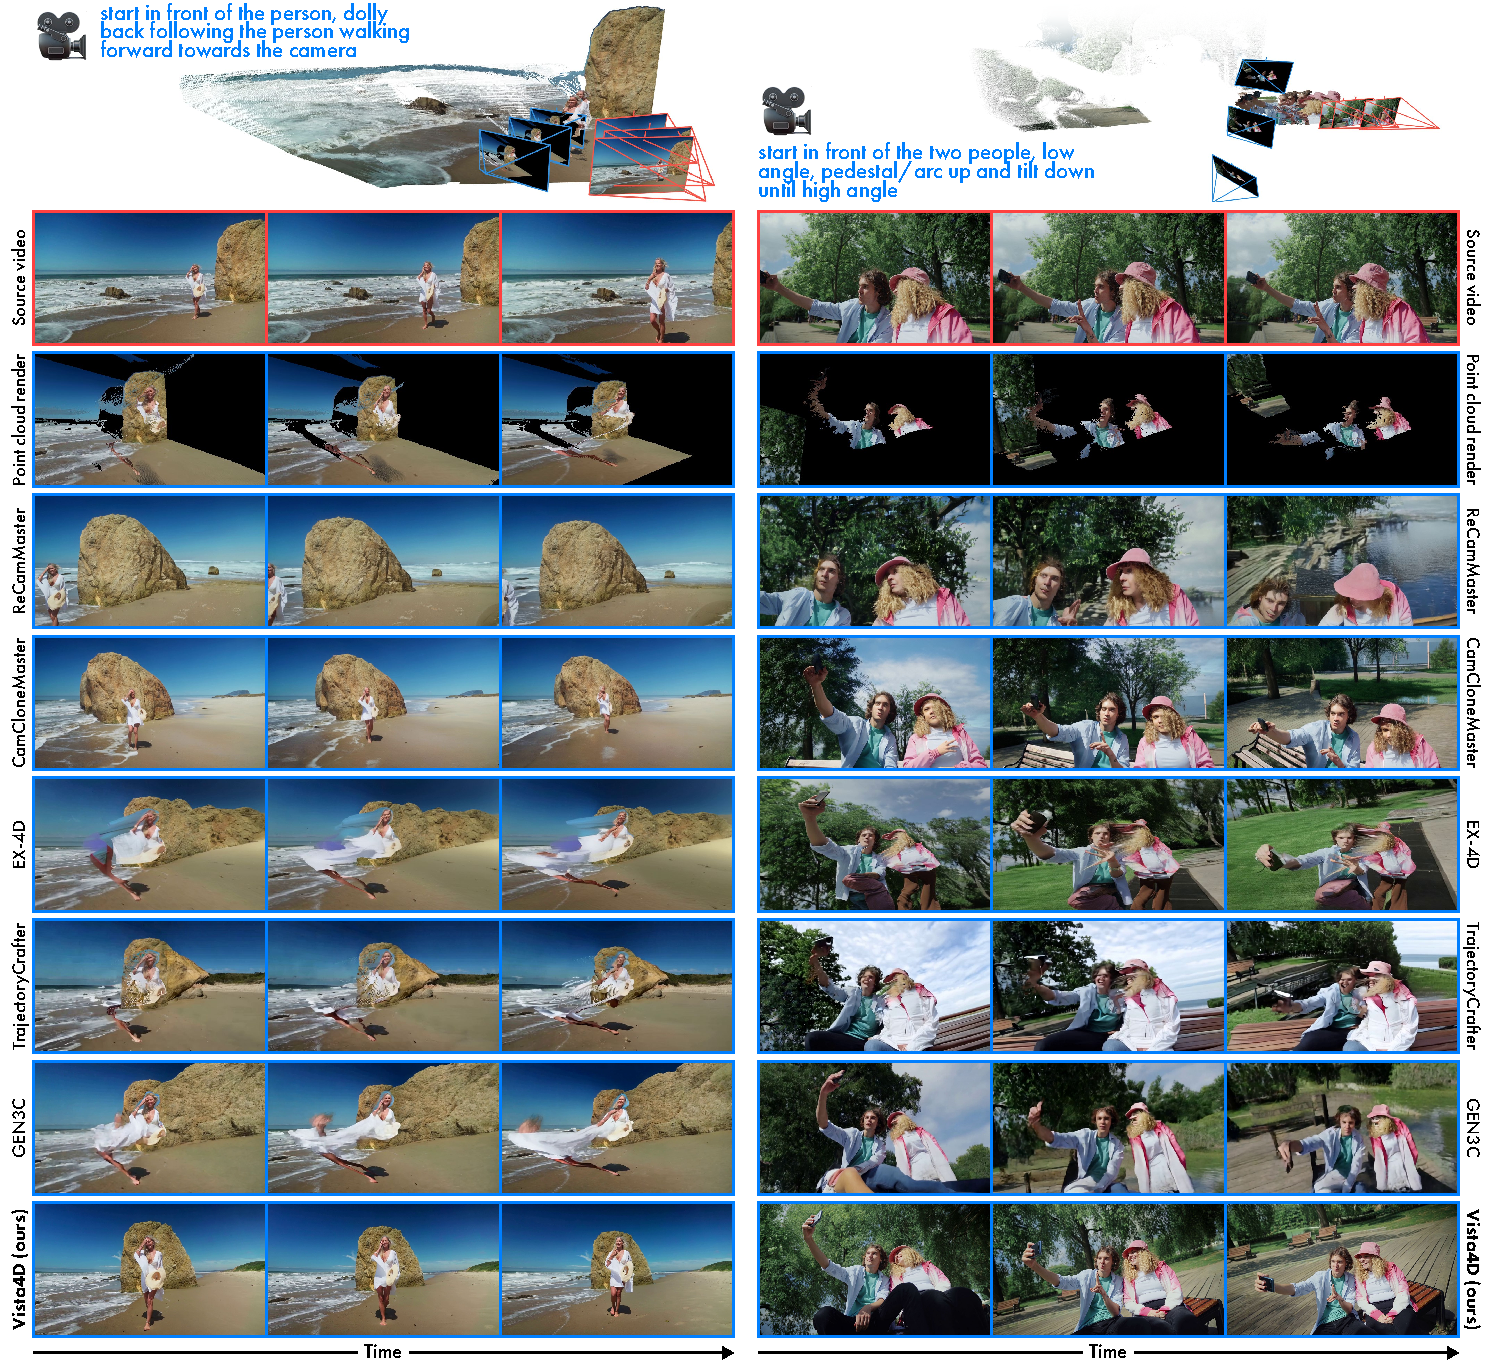
\includegraphics[width=\textwidth]{figures/mid_res/qual_comp_1.pdf}
    \caption{\Paragraphnoskip{More qualitative comparison on real-life monocular videos, part 1/2} We show two more video reshooting examples of \methodname compared to baselines: ReCamMaster \cite{bai2025recammaster}, CamCloneMaster \cite{luo2025camclonemaster}, EX-4D \cite{hu2025ex4d}, TrajectoryCrafter \cite{yu2025trajcraft}, and GEN3C \cite{ren2025gen3c}. We encourage viewing these comparisons as videos on our \projectpage, which also contains more comparisons.}
    \label{fig:qual_comp_1}
\end{figure*}

\begin{figure*}
    \centering
    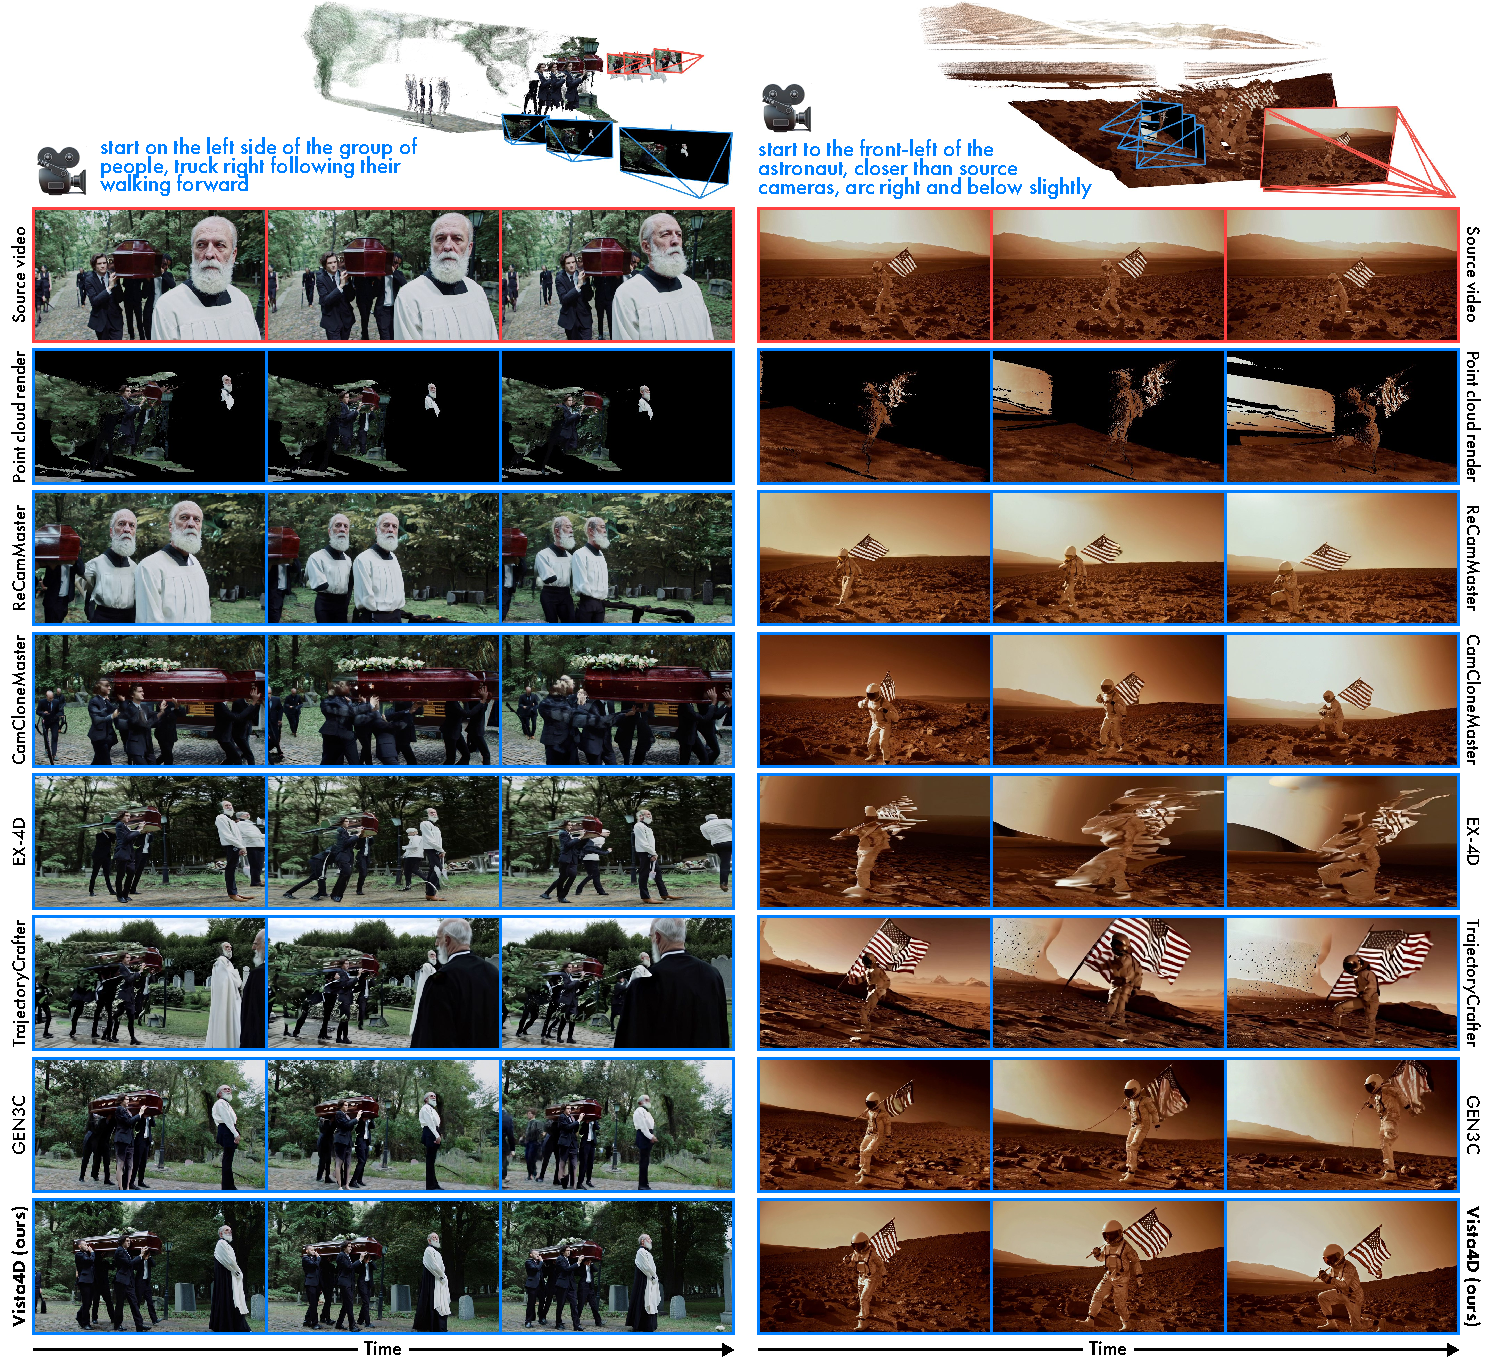
\includegraphics[width=\textwidth]{figures/mid_res/qual_comp_2.pdf}
    \caption{\Paragraphnoskip{More qualitative comparison on real-life monocular videos, part 2/2} We show two more video reshooting examples of \methodname compared to baselines: ReCamMaster \cite{bai2025recammaster}, CamCloneMaster \cite{luo2025camclonemaster}, EX-4D \cite{hu2025ex4d}, TrajectoryCrafter \cite{yu2025trajcraft}, and GEN3C \cite{ren2025gen3c}. We encourage viewing these comparisons as videos on our \projectpage, which also contains more comparisons.}
    \label{fig:qual_comp_2}
\end{figure*}

\Paragraph{Comparison to baselines}
We show more qualitative comparisons of \methodname to baselines ReCamMaster \cite{bai2025recammaster}, CamCloneMaster \cite{luo2025camclonemaster}, EX-4D \cite{hu2025ex4d}, TrajectoryCrafter \cite{yu2025trajcraft}, and GEN3C \cite{ren2025gen3c}, in Figures \ref{fig:qual_comp_1} and \ref{fig:qual_comp_2}. \methodname consistently has better preservation of the source video, more accurate camera control, and better video fidelity. Even more comparisons to baselines can be found as videos on our \projectpage.

\begin{figure*}
    \centering
    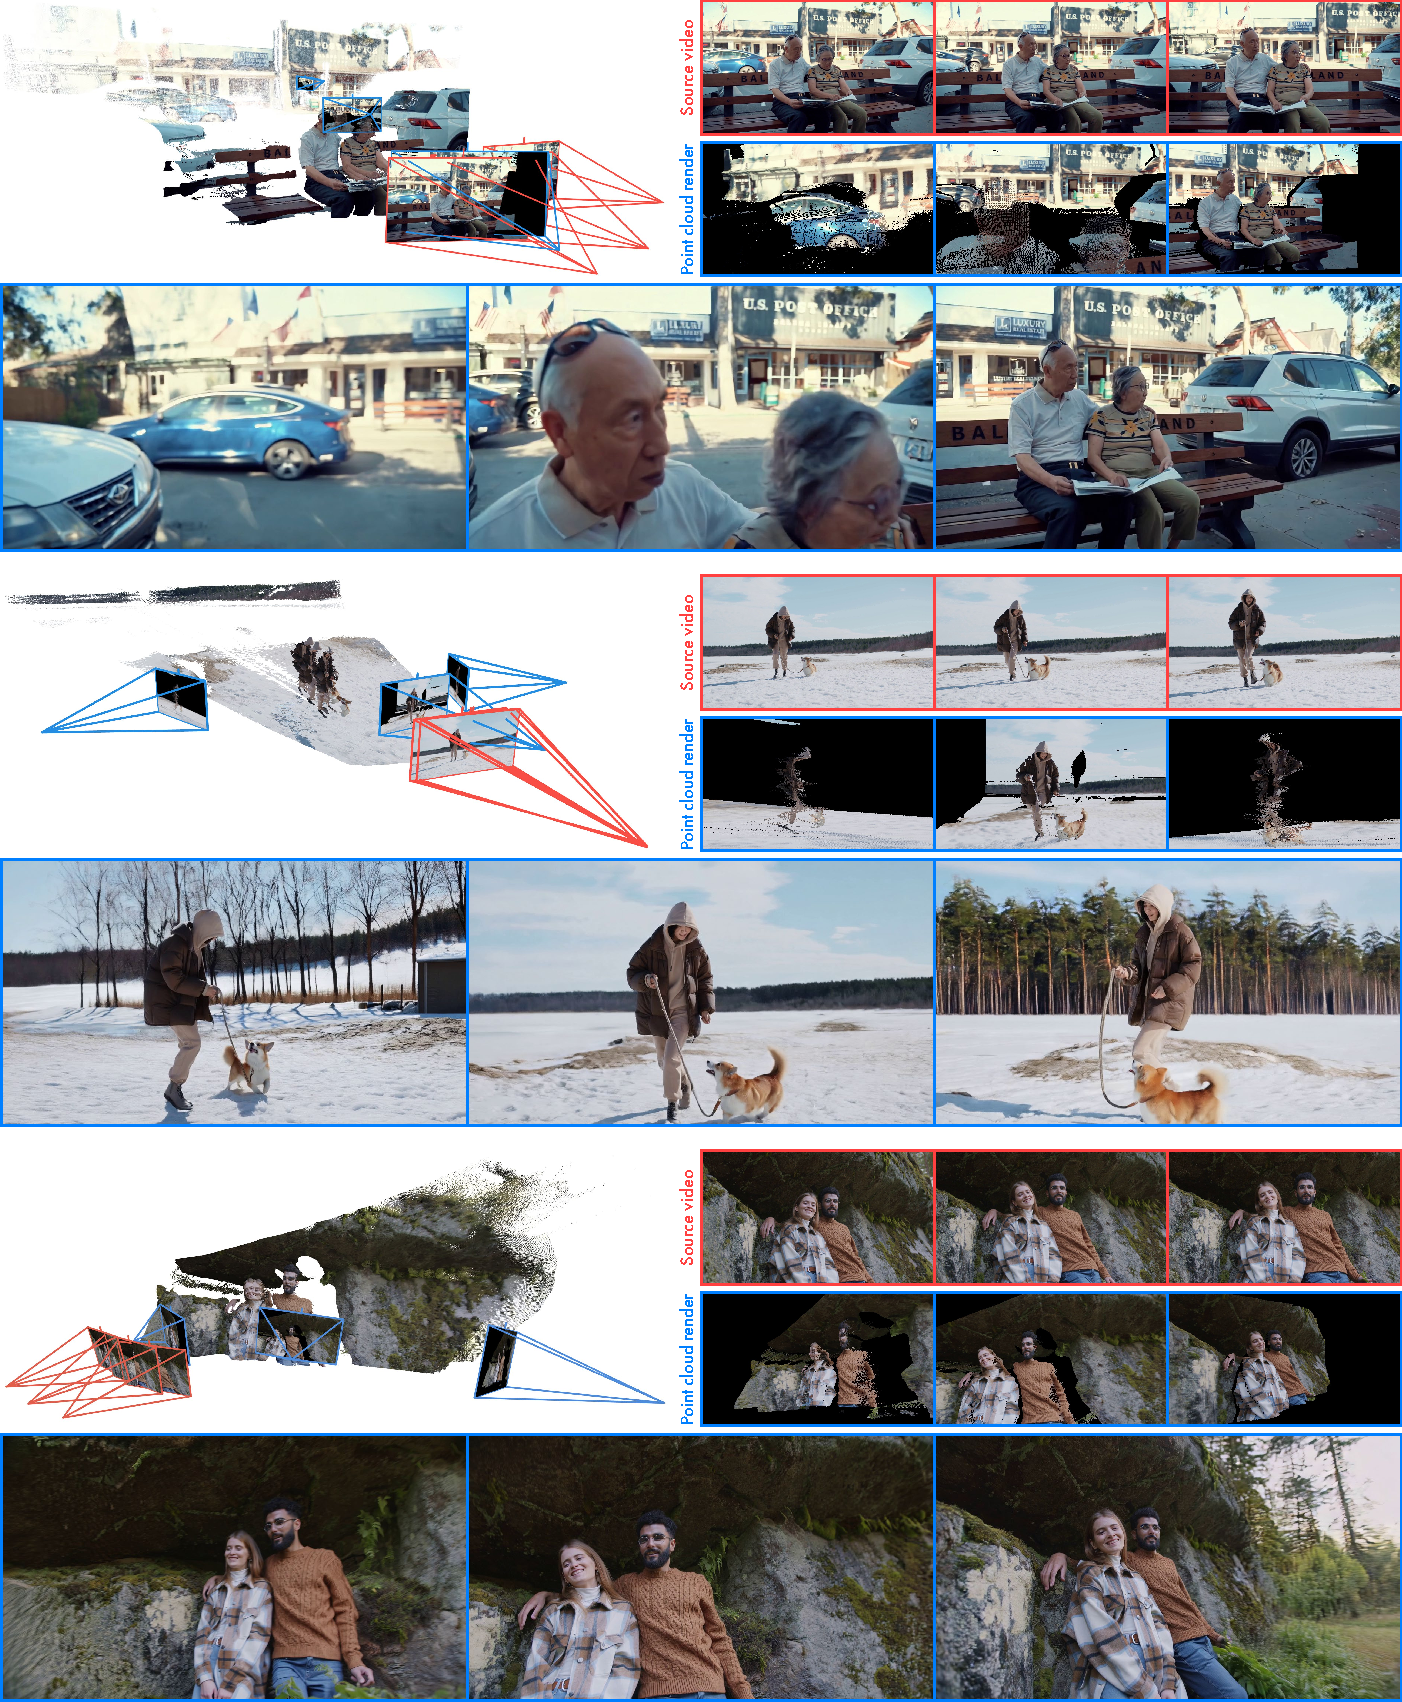
\includegraphics[width=\textwidth]{figures/mid_res/results_720p.pdf}
    \caption{\Paragraphnoskip{Video reshooting results at 720p} We show video reshooting results of \methodname with our $1280 \times 720$ finetuned checkpoint. More 720p results of our method can be found as videos on our \projectpage.}
    \label{fig:results_720p}
\end{figure*}

\Paragraph{Video reshooting at 720p} Figure \ref{fig:results_720p} shows video reshooting results of \methodname with our $1280 \times 720$ finetuned checkpoint. More 720p video reshooting results can be found on our \projectpage.

\subsection{More application results and details}

\begin{figure*}
    \centering
    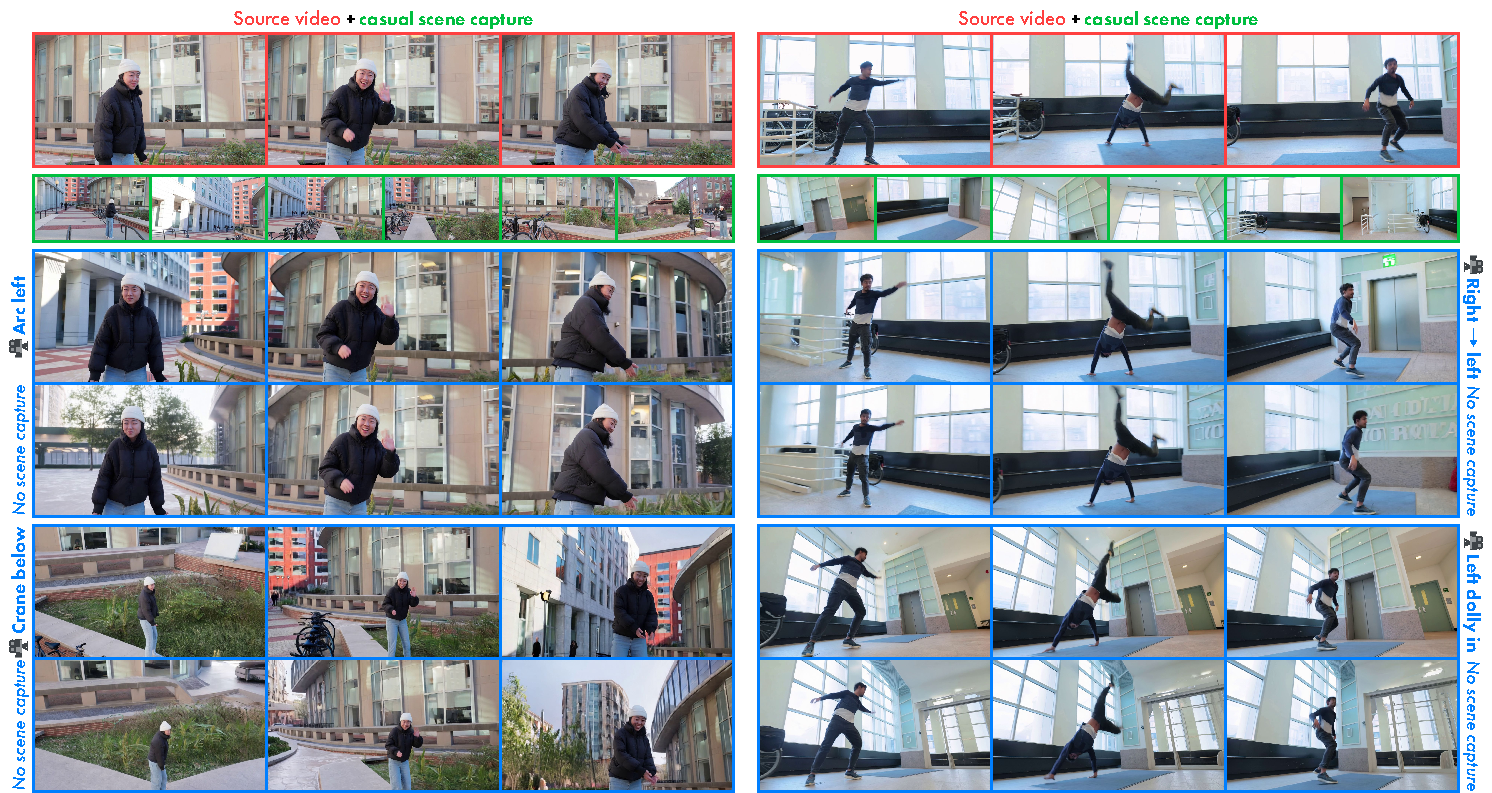
\includegraphics[width=\textwidth]{figures/mid_res/multiview_1.pdf}
    \caption{\Paragraphnoskip{More dynamic scene expansion results} We show more dynamic scene expansion results, where we incorporate additional scene information from casual scene captures by doing joint 4D reconstruction of these frames with the source video. We encourage viewing these results (and more) as videos on our \projectpage.}
    \label{fig:multiview_1}
\end{figure*}

\Paragraph{Dynamic scene expansion}
We show more dynamic scene expansion results in Figure \ref{fig:multiview_1}, where we incorporate additional scene information from casual scene captures by doing joint 4D reconstruction of these frames with the source video. We encourage viewing these results (and more) as videos on our \projectpage.

\begin{figure*}
    \centering
    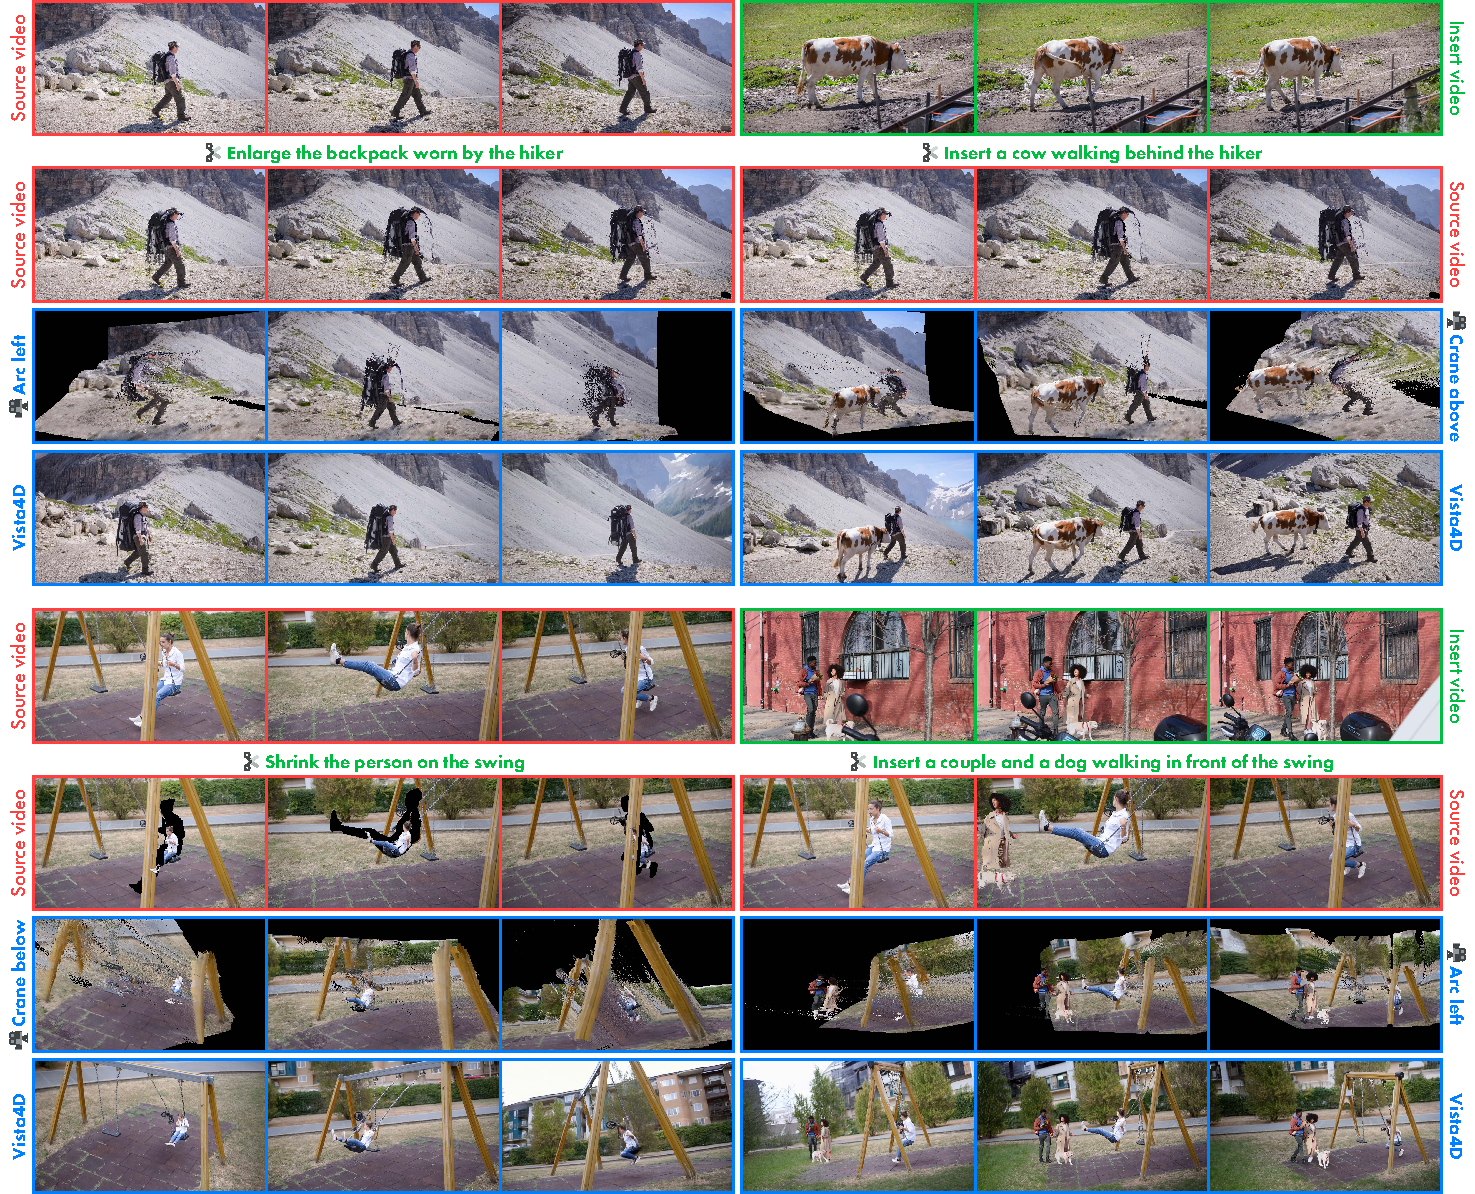
\includegraphics[width=\textwidth]{figures/low_res/scene_recomp_1.pdf}
    \caption{\Paragraphnoskip{More 4D scene recomposition results} We show more 4D scene recomposition results by directly manipulating the 4D point cloud. To prevent conditioning conflicts between the \emph{unedited} source video and render of the \emph{edited} point cloud, we instead condition on the \emph{edited} source video which is just the edited point cloud rendered from the source cameras. We encourage viewing these results (and more) as videos on our \projectpage.}
    \label{fig:scene_recomp_1}
\end{figure*}

\Paragraph{4D scene recomposition}
We show more 4D scene recomposition results in Figure \ref{fig:scene_recomp_1}. To prevent conditioning conflicts between the \emph{unedited} source video and render of the \emph{edited} point cloud, we instead condition on the \emph{edited} source video which is just the edited point cloud rendered from the source cameras without static pixel temporal persistence. Since, during training, we still include the source video condition for monocular videos, where the source video is the first render $\mathbf{X}^\tgtsrc$ of double reprojection, our model is also robust to holes and slight artifacts in the source video which the \emph{edited} source videos can contain. We encourage viewing these results (and more) as videos on our \projectpage.

\begin{figure*}
    \centering
    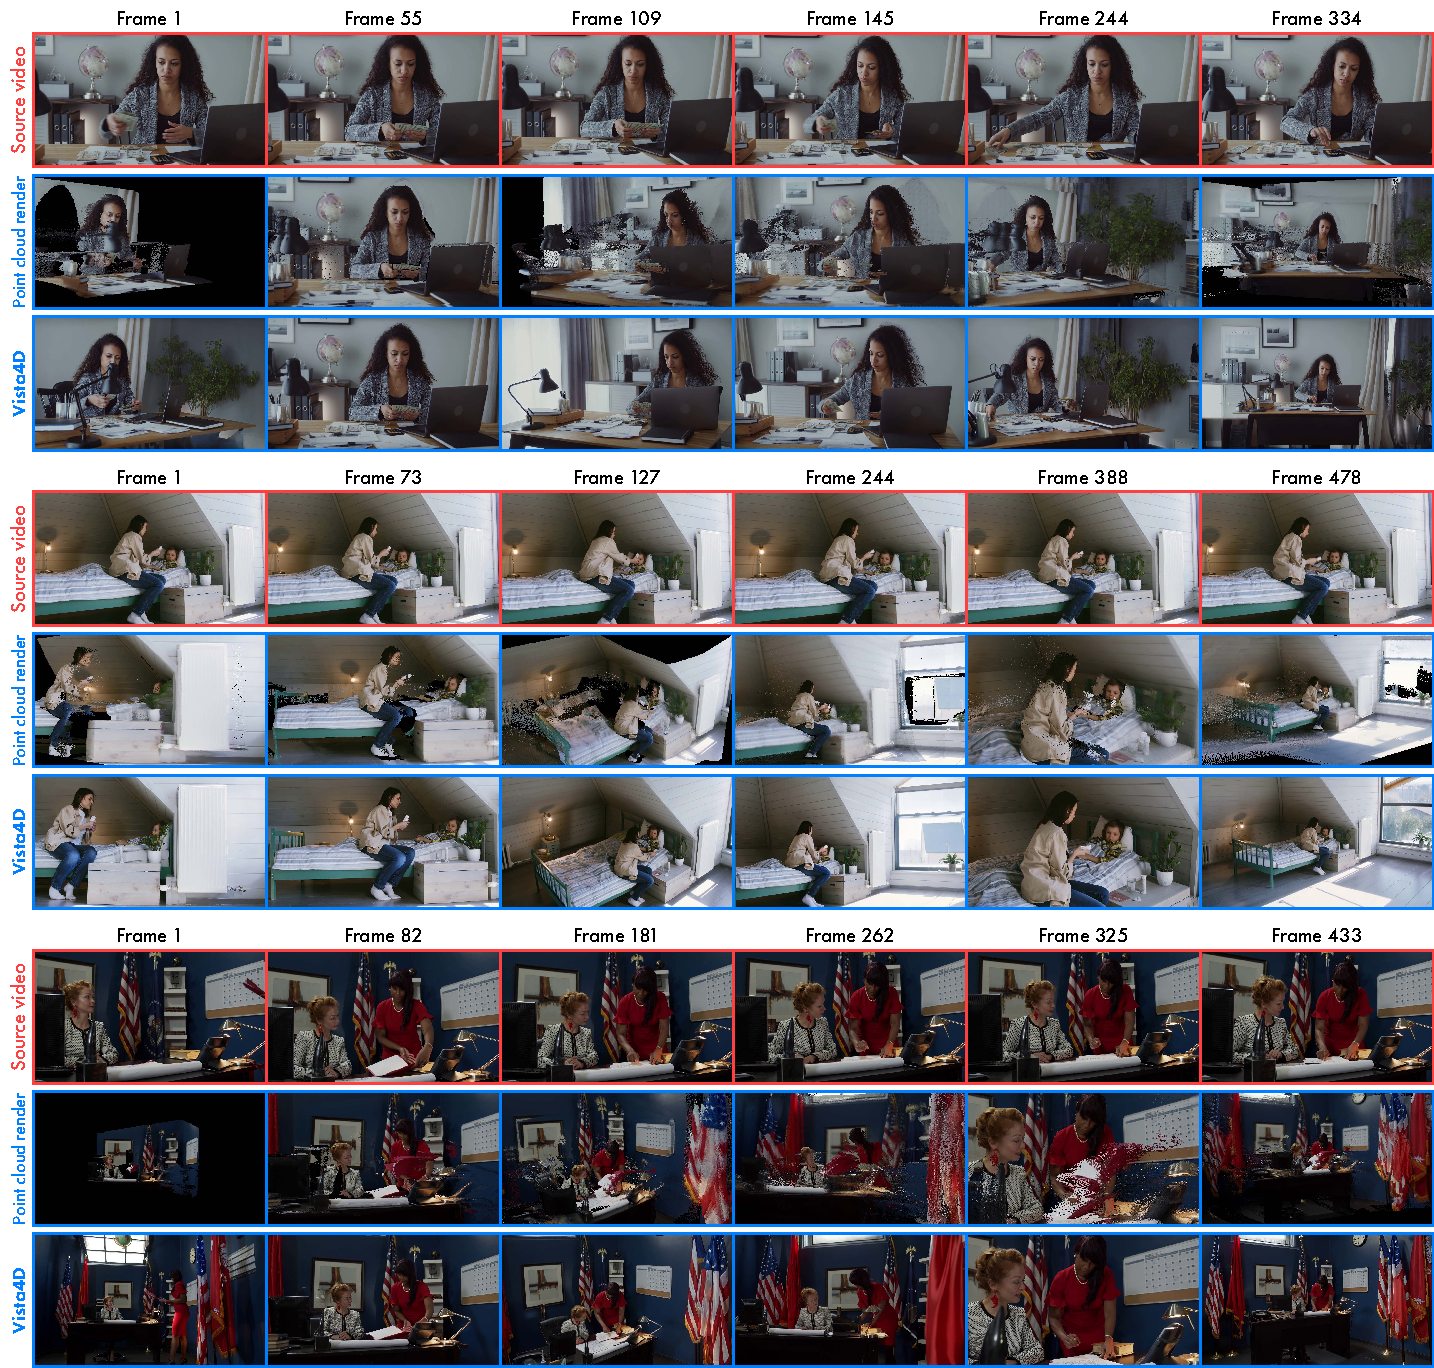
\includegraphics[width=\textwidth]{figures/low_res/long_video_1.pdf}
    \caption{\Paragraphnoskip{More long video inference results} We show more results of inference on long videos. To do so, we chunk the source video into $49$-frame clips and run inference clip-by-clip. To explicitly preserve generated content, we continuously integrate the point cloud from the newly generated video into the existing one after each inference pass, which is visualized in the point cloud renders above. We encourage viewing these results (and more) as videos on our \projectpage.}
    \label{fig:long_video_1}
\end{figure*}

\Paragraph{Long video inference}
We show more long video inference results in Figure \ref{fig:long_video_1} and on our \projectpage. To support \methodname inference on long source videos, we chunk the source video into $49$-frame clips and run inference clip-by-clip. To hold explicit memory of generated content across clips, we need a 4D reconstruction method to continuously integrate the dynamic point cloud from the newly generated video clip into the existing one after each inference pass. We find existing autoregressive 4D reconstruction methods~\cite{wang2025cut3r, lan2025stream3r} to suffer from bad accuracy with very long videos, while the more accurate $\pi^3$~\cite{wang2025pi3} model only supports feedforward reconstruction. Therefore, we extend $\pi^3$ to support chunk-autoregressive inference by subsampling a constant number of frames from the existing frames and concatenating them with the newly generated frames for joint reconstruction. We then fit the existing-frame part of the predicted cameras to the known camera parameters using Umeyama alignment \cite{umeyama2002least}, while registering the new camera poses and point clouds from the generated frames to the 4D reconstruction result.

\begin{figure*}
    \centering
    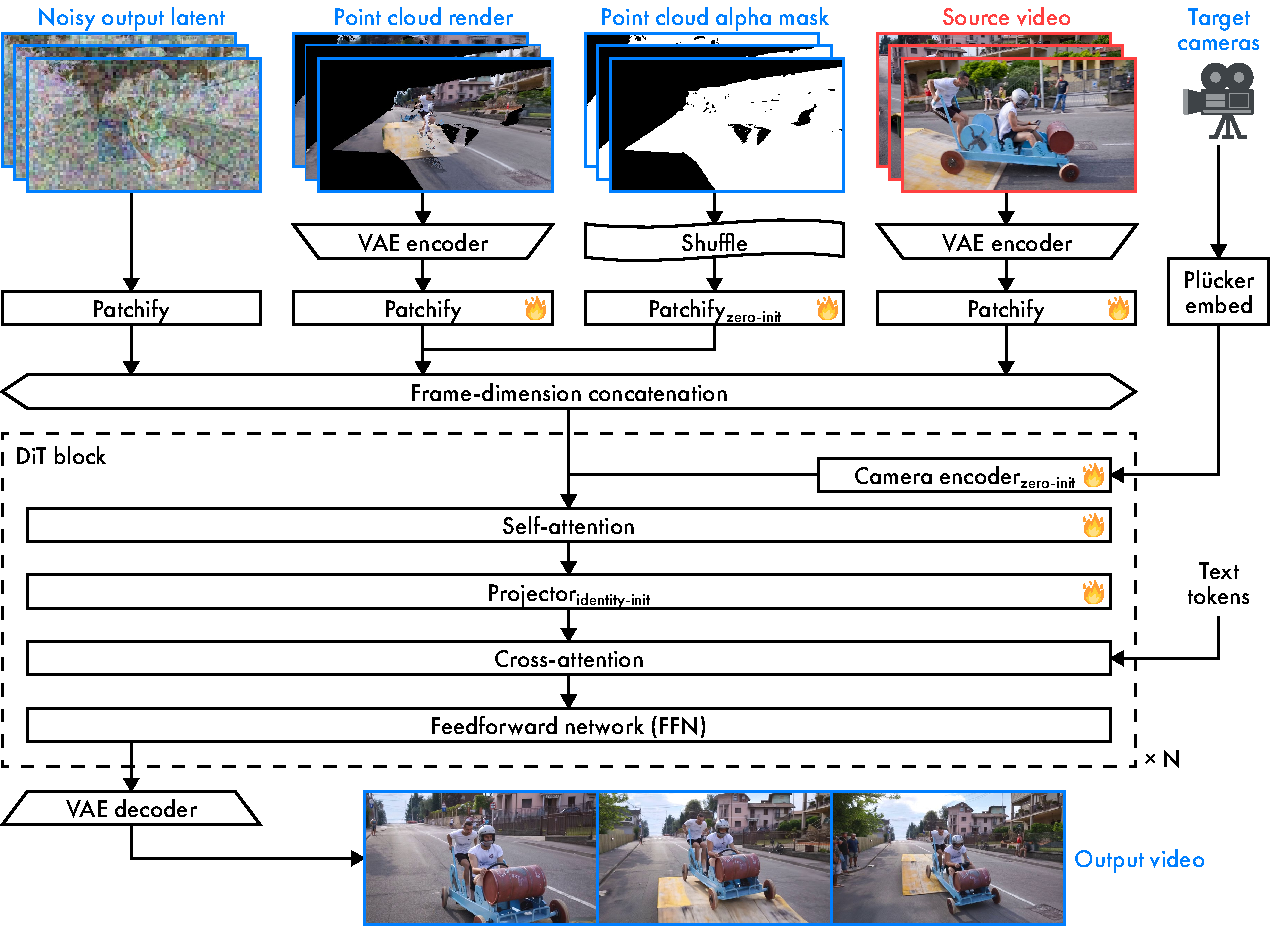
\includegraphics[width=0.75\textwidth]{figures/mid_res/architecture.pdf}
    \caption{\Paragraphnoskip{Model architecture} The above diagram shows the model architecture for \methodname. The fire icon indicates trainable parameters. We build upon \texttt{Wan2.1-T2V-14B} \cite{wan2025}, and we omit timestep conditioning, text prompt to token embedding, modulation, layer normalization, output unshuffle, and diffusion model denoising in the diagram for simplicity. All patchify layers are initialized from the base video model besides that of the point cloud render alpha mask, which is zero-initialized. The camera encoder is zero-initialized, and the projector after self-attention is initialized as the identity affine transformation.}
    \label{fig:architecture}
\end{figure*}

\section{Model architecture details} \label{supp:architecture}

The model architecture for \methodname builds upon a text-to-video (T2V) diffusion model, namely \texttt{Wan2.1-T2V-14B} \cite{wan2025}. We finetune the T2V model to be additionally conditioned on an input source video, target cameras, point cloud render in said target cameras, and the point cloud render's alpha mask, where the model produces the output video which synthesizes the dynamic scene represented by the source video from the given target cameras. A diagram of our model architecture can be found in Figure \ref{fig:architecture}.

We first encode the source video and point cloud render into latents with the VAE, while token shuffling the point cloud render's alpha mask to match the latent space height and width. We initialize patchify layers for the source video and point cloud render from the base video model, and we zero-initialize the alpha mask's patchify layer to sum the resulting tokens with that of the point cloud render. We then concatenate the source video and point cloud render tokens with that of the noisy target along the frame dimension.

For each DiT block, we inject the target cameras as Pl\"{u}cker embeddings \cite{kuang2024collaborative, he2025cameractrl, xu2025virtuallybeing} via a zero-initialized linear camera projection which is summed with the hidden states before self-attention. After self-attention, we additionally project the hidden states with an identity-initialized affine transform before cross-attention and feedforward network (FFN), inspired by ReCamMaster \cite{bai2025recammaster}. We train the camera encoders, self-attention, projector, and all patchify layers besides that of the noisy output latent, while freezing all other parameters.

\section{Dataset and training details}
\label{sec:supp_train_data}

\subsection{Training dataset}

We train with a combination of multiview and monocular video datasets. For multiview videos, MultiCamVideo \cite{bai2025recammaster} is a synthetic time-synchronized dynamic multiview dataset from ReCamMaster. For monocular videos, \texttt{OpenVidHD-0.4M} \cite{nan2025openvid} is a filtered and labeled monocular video dataset of internet videos. The sampling ratio of multiview and monocular videos is $1:1$. More details for how we process each dataset are below.

\Paragraph{MultiCamVideo} MultiCamVideo renders its scenes at fixed camera intrinsics, and the dataset contains four unique intrinsics. For each of these intrinsics, we select the first $512$ (out of $3400$) scenes. We run 4D reconstruction with STream3R \cite{lan2025stream3r} with a moving window size of $128$ so all ten views of MultiCamVideo can fit on a single GPU. Then, we input the frames in a frame-first (\ie, we stream in all views for the current frame before moving onto the next frame) as opposed to a view-first (\ie, we stream in all frames for the current view before moving onto the next view) order. Formally, the frame-first order rearranges the tensor from \texttt{v f h w 3} to \texttt{(f v) h w 3}, where \texttt{v} is the view dimension. We do so as we find the frame-first order better ensures rough foreground/dynamic subject depth alignment between different views (as the relative scale of foreground subjects to the background scene is inherently ambiguous) since STream3R is processing different views from the same frame in close proximity due to the moving window. Though this results in temporal jittering of the predicted target cameras, we simply smooth the target camera intrinsics and extrinsics with a Gaussian kernel at the end as MultiCamVideo only renders with smooth cameras. We caption the videos with a combination of \texttt{cogvlm2-video-llama3-chat} and \texttt{cogvlm2-llama3-caption} \cite{hong2024cogvlm2, yang2025cogvideox}.

\Paragraph{\texttt{OpenVidHD-0.4M}} We select a random 60K subset from the dataset. As OpenVid provides high-level camera movement annotations, we filter for videos that are not labeled \texttt{"static"} to better learn more dynamic target cameras. We further filter out video cuts in the downloaded videos with \texttt{PySceneDetect} \cite{castellano2025pyscenedetect}. We use captions from the dataset.

Inspired by Uni4D \cite{yao2025uni4d}, we automatically segment dynamic pixels from our all datasets to produce the static pixel masks for constructing our temporally-persistent point clouds. For each video, we obtain semantic classes with RAM \cite{zhang2023ram} and prompt \texttt{Llama-3.1-8B-Instruct} \cite{llama2024llama3} to filter for subjects/nouns that would reasonably be dynamic in a video. With the list of keywords, we segment per-frame dynamic pixels with Grounded SAM 2 \cite{ravi2024sam2, ren2024groundingdino, ren2024groundedsam} and invert the result to obtain our static pixel masks.

\subsection{Training details}

We finetune \texttt{Wan2.1-T2V-14B} \cite{wan2025} for our main checkpoint. We do $10\%$ random drops each for the source video, point cloud render, prompt, and camera conditioning. When dropping the source video and/or the point cloud render, we set their latents as Gaussian noise following ReCamMaster \cite{bai2025recammaster} and zero their corresponding alpha masks.

\Paragraph{Removing the matching-first-frame constraint}
Most of the baselines that we compare to in this paper assume that the first frame of the source and target cameras (intrinsics and extrinsics) match. Doing so enables most of them to finetune from an image-to-video (I2V) as opposed to text-to-video (T2V) diffusion model to utilize the strong preservation and geometry priors of the first-frame-conditioned model. Additionally, for implicit-prior methods, this enables the camera conditioning to be relative to the first source video frame as opposed to some translation- and scale-invariant world space. We do not have this constraint for \methodname, which is achieved by both using a text-to-video model and also data processing. Notably, since MultiCamVideo always has matching source and target camera first frames, we do $50\%$ random time-reversal of the source and target videos together.

\Paragraph{Finetuning I2V diffusion models for long video inference}
We also finetune \texttt{Wan2.1-I2V-14B} \cite{wan2025} for long video inference, as we find the first-frame condition helpful for maintaining visual consistency between consecutive inference chunks. We train with the exact same dataset and simply also condition the model on the first frame of the target video, even if said first frame does not match that of the source video. We do $30\%$ random drop for the image condition to strengthen the point cloud render's influence, as we otherwise observe poorer camera control during preliminary experiments when the model more heavily relies on the image condition. We also apply noise-augmentation condition on the image latent to reduce quality degradation with more inference chunks. Namely, given the image condition $\mathbf{X}^\img$, we obtain the augmented $\overline{\vec{X}^\img} = (1 - \alpha) \vec{X}^\img + \alpha \boldsymbol{\epsilon}$ where $\alpha = 0.05$ and $\boldsymbol{\epsilon} \sim \NN(0, \vec{I})$. During inference, we use our T2V-finetuned checkpoint for the first $49$-frame clip and I2V-finetuned checkpoint for all subsequent clips.

\section{Evaluation dataset and user study details} \label{supp:eval_user}

We construct a $110$ video-camera pair evaluation dataset for quantitative evaluations and our user study. We select $13$ videos from DAVIS \cite{perazzi2016davis} and $38$ videos from Pexels \cite{pexels2025} which are high quality and contain dynamic scene and/or camera motion. We then design two to three target camera trajectories and zooms for each video with our camera design UI. We reconstruct all videos with $\pi^3$ \cite{wang2025pi3} and manually annotate keywords for segmenting dynamic pixels with Grounded SAM 2 \cite{ravi2024sam2, ren2024groundingdino, ren2024groundedsam}. We caption all videos with a combination of \texttt{cogvlm2-llama3-caption} \cite{yang2025cogvideox} and Gemini 2.5 Pro \cite{2025gemini25}. We release the evaluation dataset and our annotations with our public code and weights release, which can be found on our \projectpage.

\begin{figure*}
    \centering
    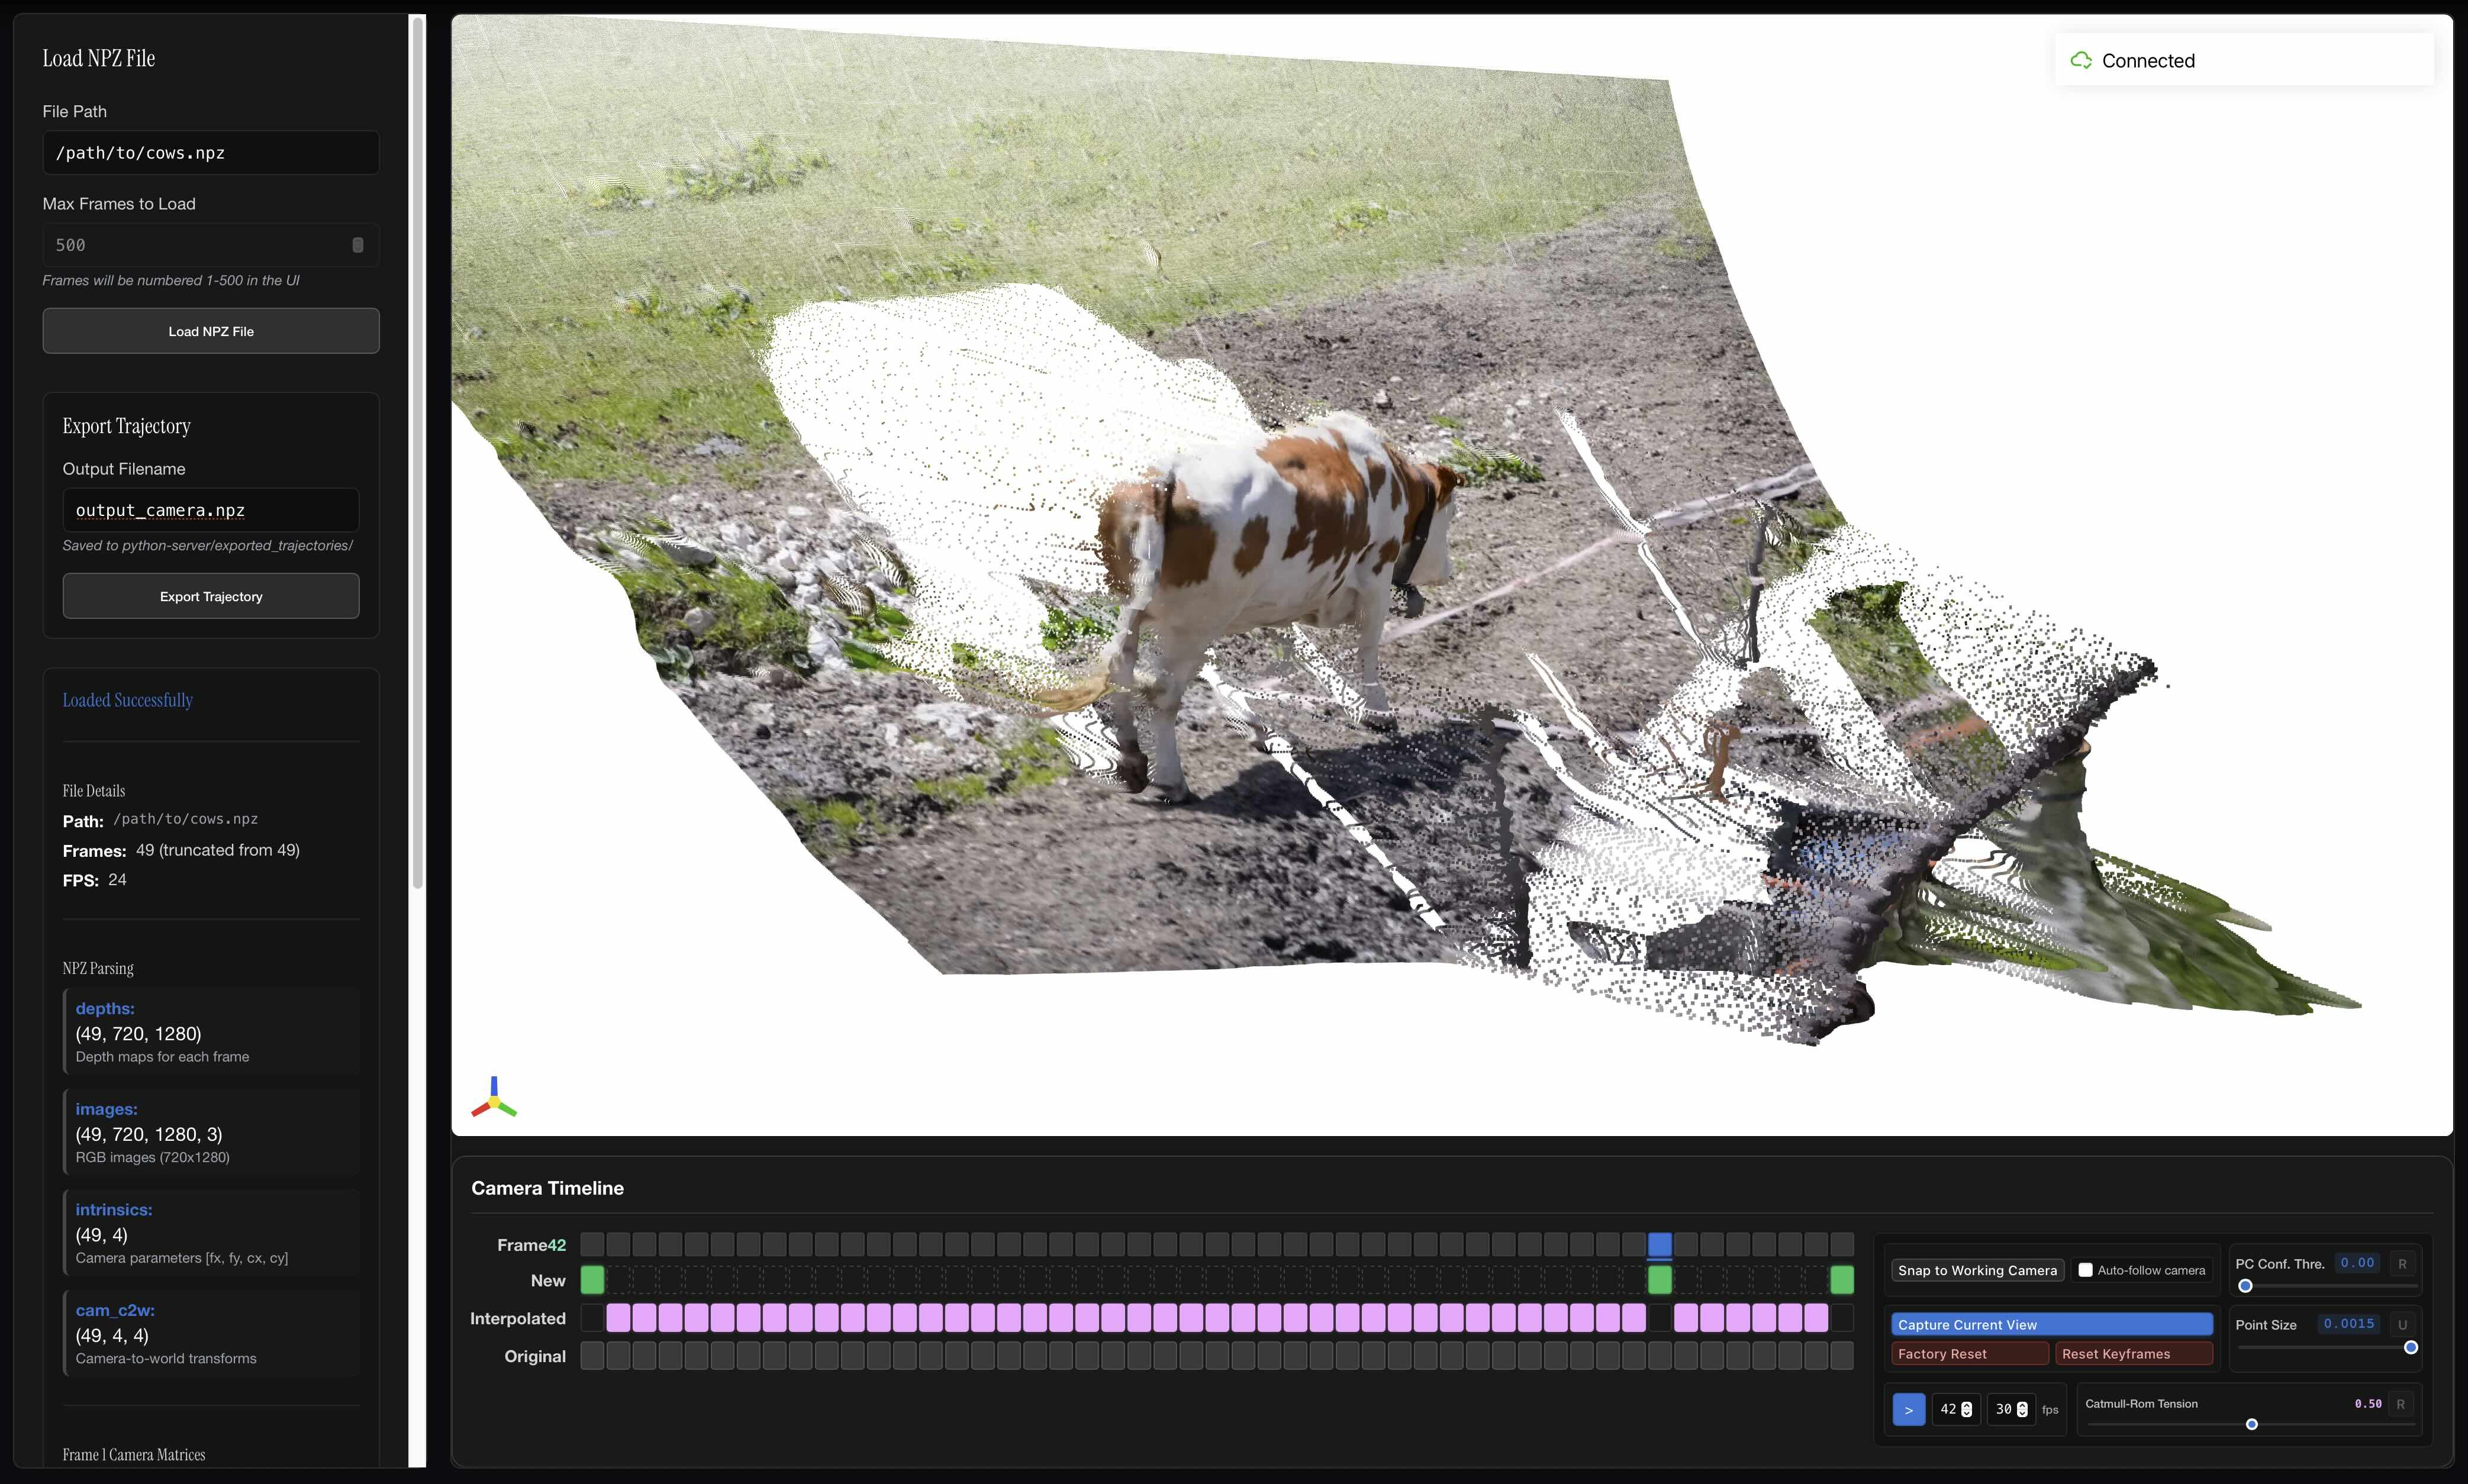
\includegraphics[width=0.75\textwidth]{figures/mid_res/camera_ui.jpg}
    \caption{\Paragraphnoskip{Camera design UI} The above screenshot shows our current camera design UI, built on top of Viser \cite{yi2025viser}. Users can set camera intrinsics and extrinsics keyframes and interpolation tension/smoothness, while being able to preview the 4D reconstructed point cloud from their defined target cameras in real time.}
    \label{fig:camera_ui}
\end{figure*}

\Paragraph{Camera design UI}
We build an interface for easily defining target cameras given the 4D reconstruction of a source video, built on top of Viser \cite{yi2025viser}, and a screenshot of which can be found in Figure \ref{fig:camera_ui}. Currently, users can set camera intrinsics and extrinsics keyframes and interpolation tension/smoothness, while being able to preview their defined target cameras when playing back the video/4D point cloud. As the UI simply outputs camera intrinsics and extrinsics which are used in a separate point cloud rendering module, this does not affect temporal persistence for our final point cloud render. We release our camera design UI with our public code release, which can be found on our \projectpage.

\Paragraph{Running the baselines}
Every baseline that we compare \methodname to, besides TrajectoryCrafter \cite{yu2025trajcraft}, does not support differing first frame source and target cameras due to their data constraints or processing and/or from finetuning an I2V model (where they use the first frame of the source video as the image condition). To run inference for these baselines on video-camera pairs in our evaluation dataset which do not have matching first frame source and target cameras, we follow the following procedure first implemented in TrajectoryCrafter's codebase as \texttt{infer\_direct} mode \cite{yu2025trajcraft}: Freeze the first frame of the point cloud and move the first frame of the source camera to that of the target camera, then unfreeze the point cloud and continue the target cameras from there. In order to fairly compare with several baselines at once, we unify the quantitative evaluation at $672 \times 384$ (though we still run at each baseline's native resolutions), as several baselines do not have higher native resolutions.

\begin{table*}
    \caption{\Paragraphnoskip{Preprocessing and inference time} With user-defined dynamic keywords, inference preprocessing involves segmentation (Grounding SAM 2) and 4D reconstruction ($\pi^3$). Model inference are all 50 steps. We run everything on an NVIDIA A100 80GB.}
    \label{tab:preprocess_inference}
    \centering
    \begin{adjustbox}{max width=\linewidth}
        \begin{tabular}{l l l c c c}
            \toprule
            Method & Base model & Resolution & Segmentation (s) & 4D reconstruction (s) & Model inference (s) \\
            \midrule
            ReCamMaster & \texttt{Wan2.1-T2V-1.3B} & $832 \times 480$ & - & \multirow{2}{*}{\makecell{\textit{Implicit prior,}\\\textit{no 4D reconstruction}}} & 523.2 \\
            CamCloneMaster & \texttt{Wan2.1-T2V-1.3B} & $832 \times 480$ & - & & 1062 \\ \hline
            TrajectoryCrafter & \texttt{CogVideoX-Fun-5B} &  $672 \times 384$ & - & & 170.1 \\
            EX-4D & \texttt{Wan2.1-T2V-14B} & $672 \times 384$ & - & \multirow{4}{*}{\makecell{\textit{Explicit prior,}\\\textit{all using $\pi^3$}\\\textit{with time:}\\3.110}} & 698.9 \\
            GEN3C & \texttt{Cosmos1.0Diffusion-7BVideo2World} & $1280 \times 704$ & - & & 1110 \\
            \textbf{\methodname (ours)} & \texttt{Wan2.1-T2V-14B} & $672 \times 384$ & \multirow{2}{*}{22.75} & & 1195 \\
            \textbf{\methodname (ours)} & \texttt{Wan2.1-T2V-14B} & $1280 \times 720$ & & & 9924 \\
            \bottomrule
        \end{tabular}
    \end{adjustbox}
\end{table*}


\Paragraph{Preprocessing and inference time}
We show preprocessing and inference time of \methodname and our baselines in Table \ref{tab:preprocess_inference}, where we see that the overhead for preprocessing is negligible compared to model inference. \methodname is slower than our baselines primarily due to in-context conditioning and our slower base model. The latter may itself also contribute to higher visual quality, but as shown in our ablations in Supplementary \ref{supp:ablations}, our key designs as summarized above are the main contributors for \methodname's superior performance at specifically video reshooting.

\begin{figure*}
    \centering
    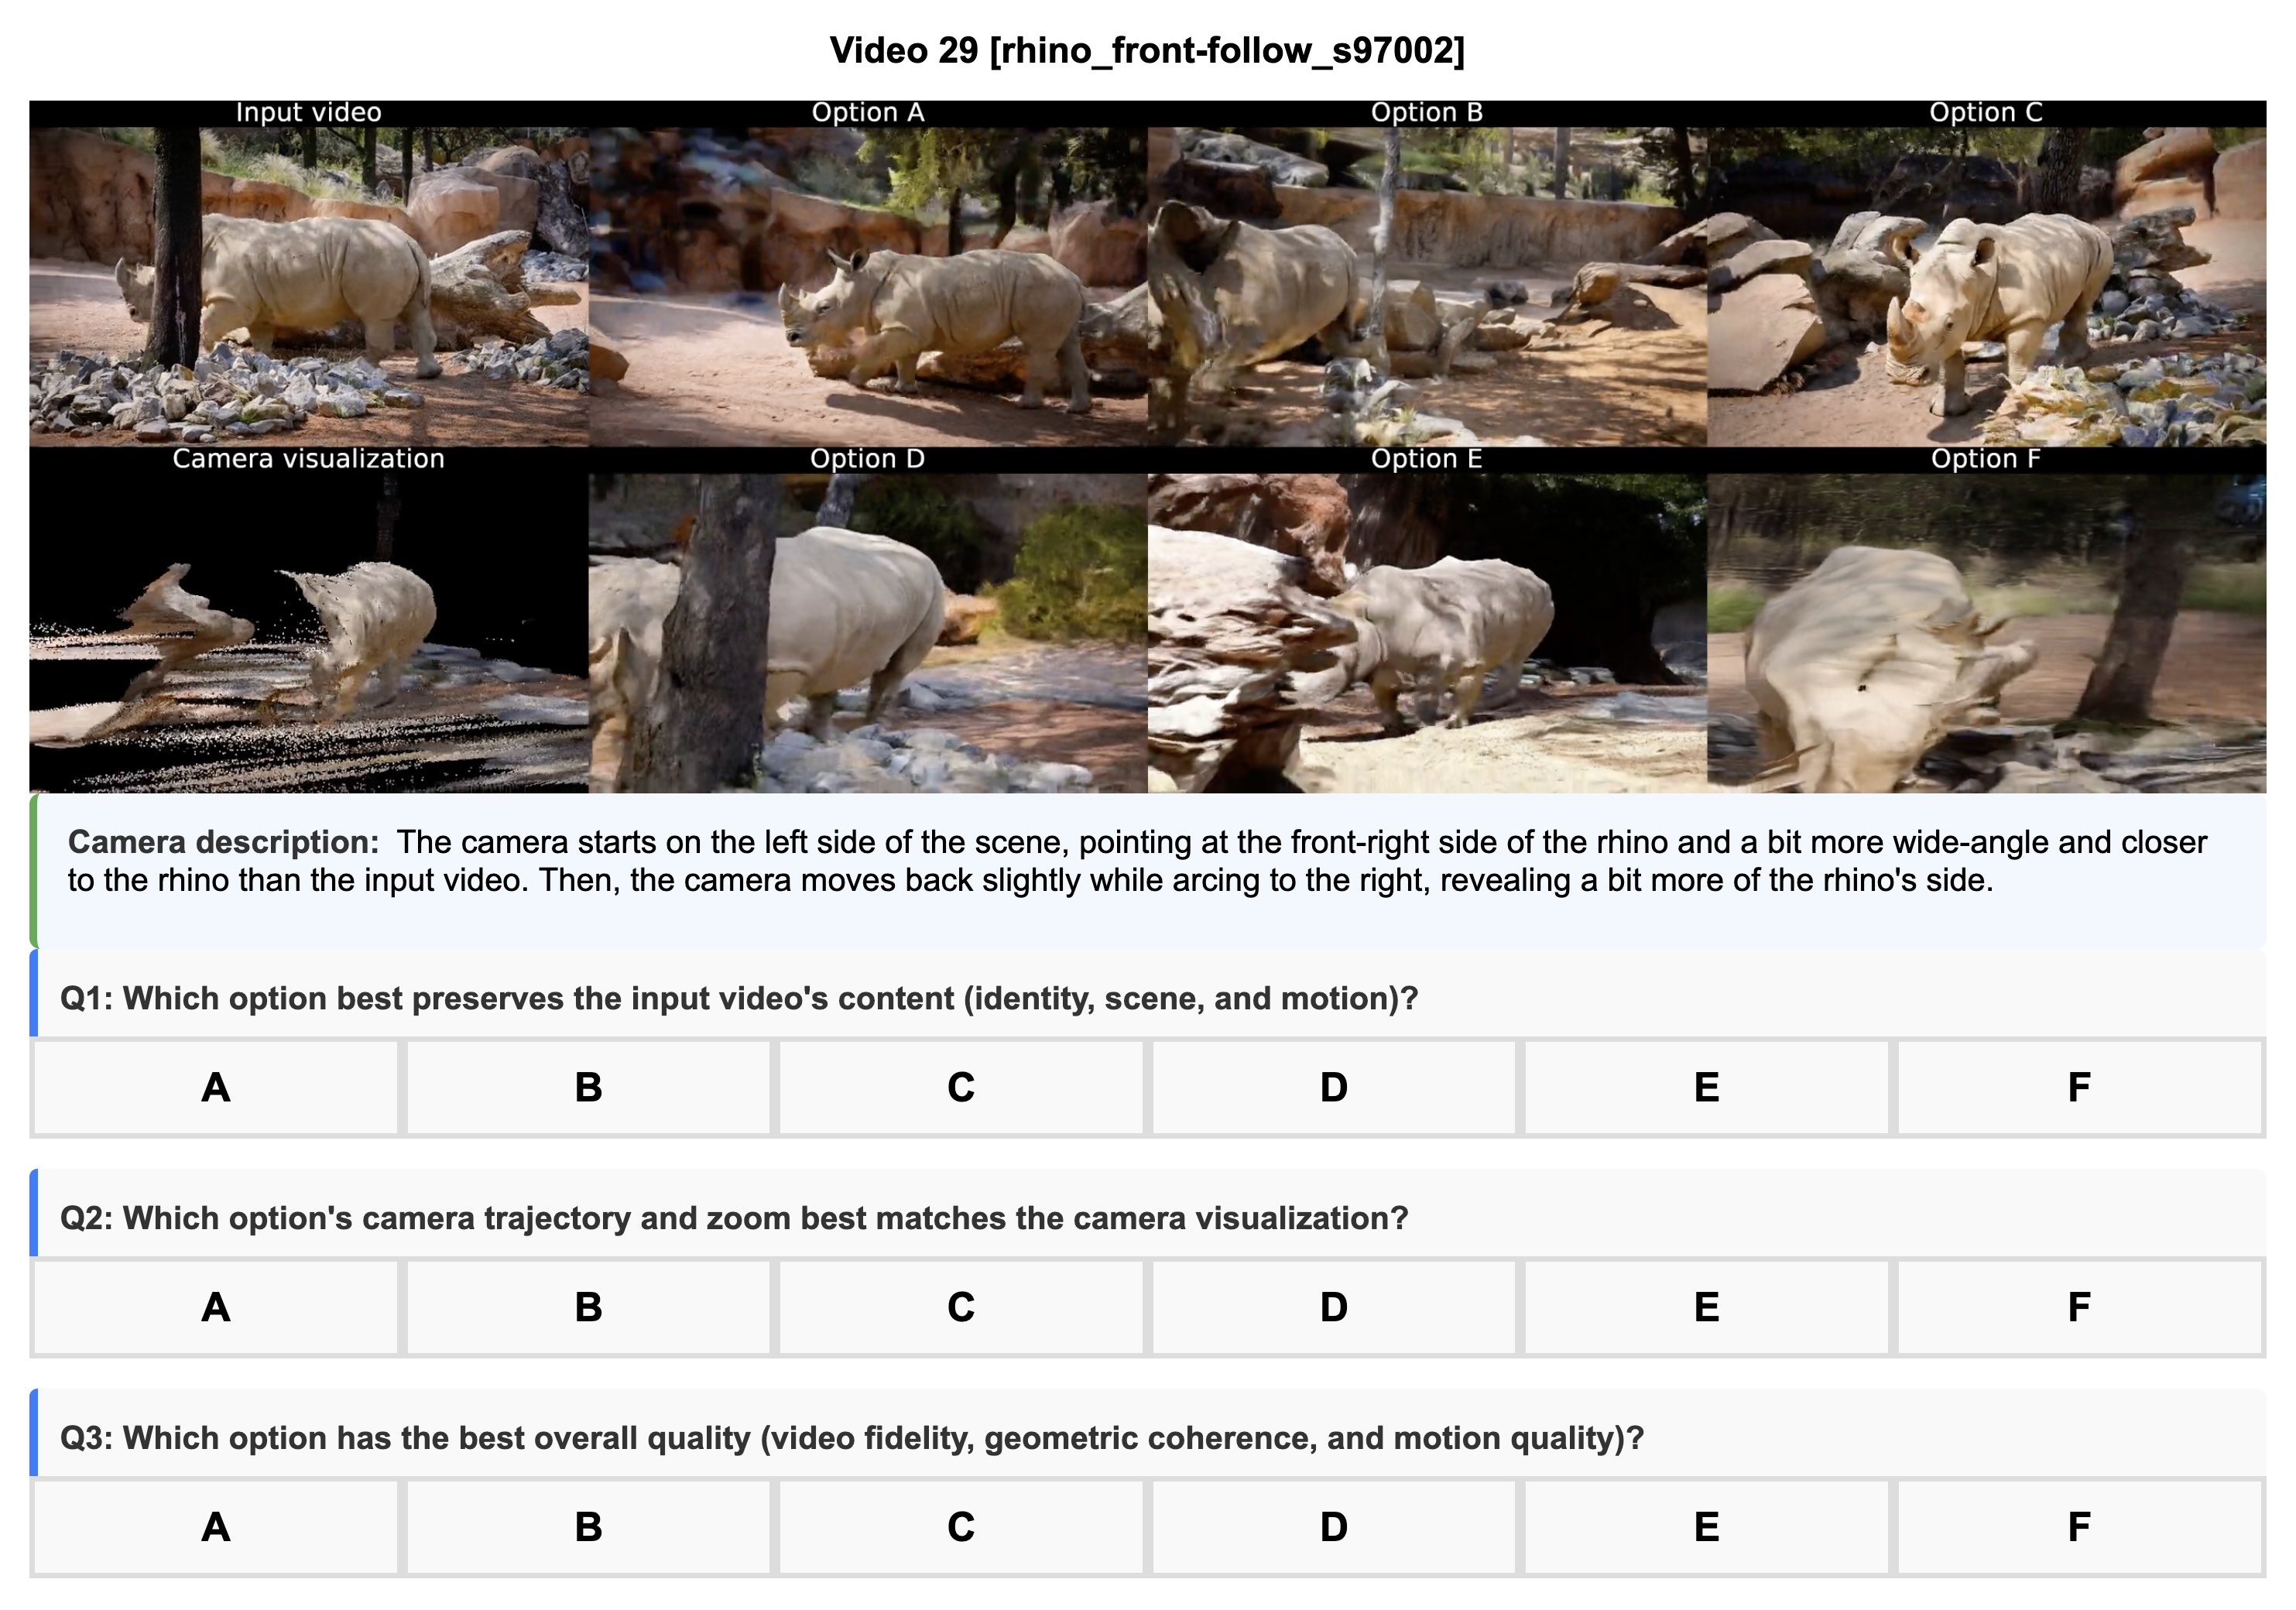
\includegraphics[width=0.49\textwidth]{figures/mid_res/user_study_rhino.jpg}
    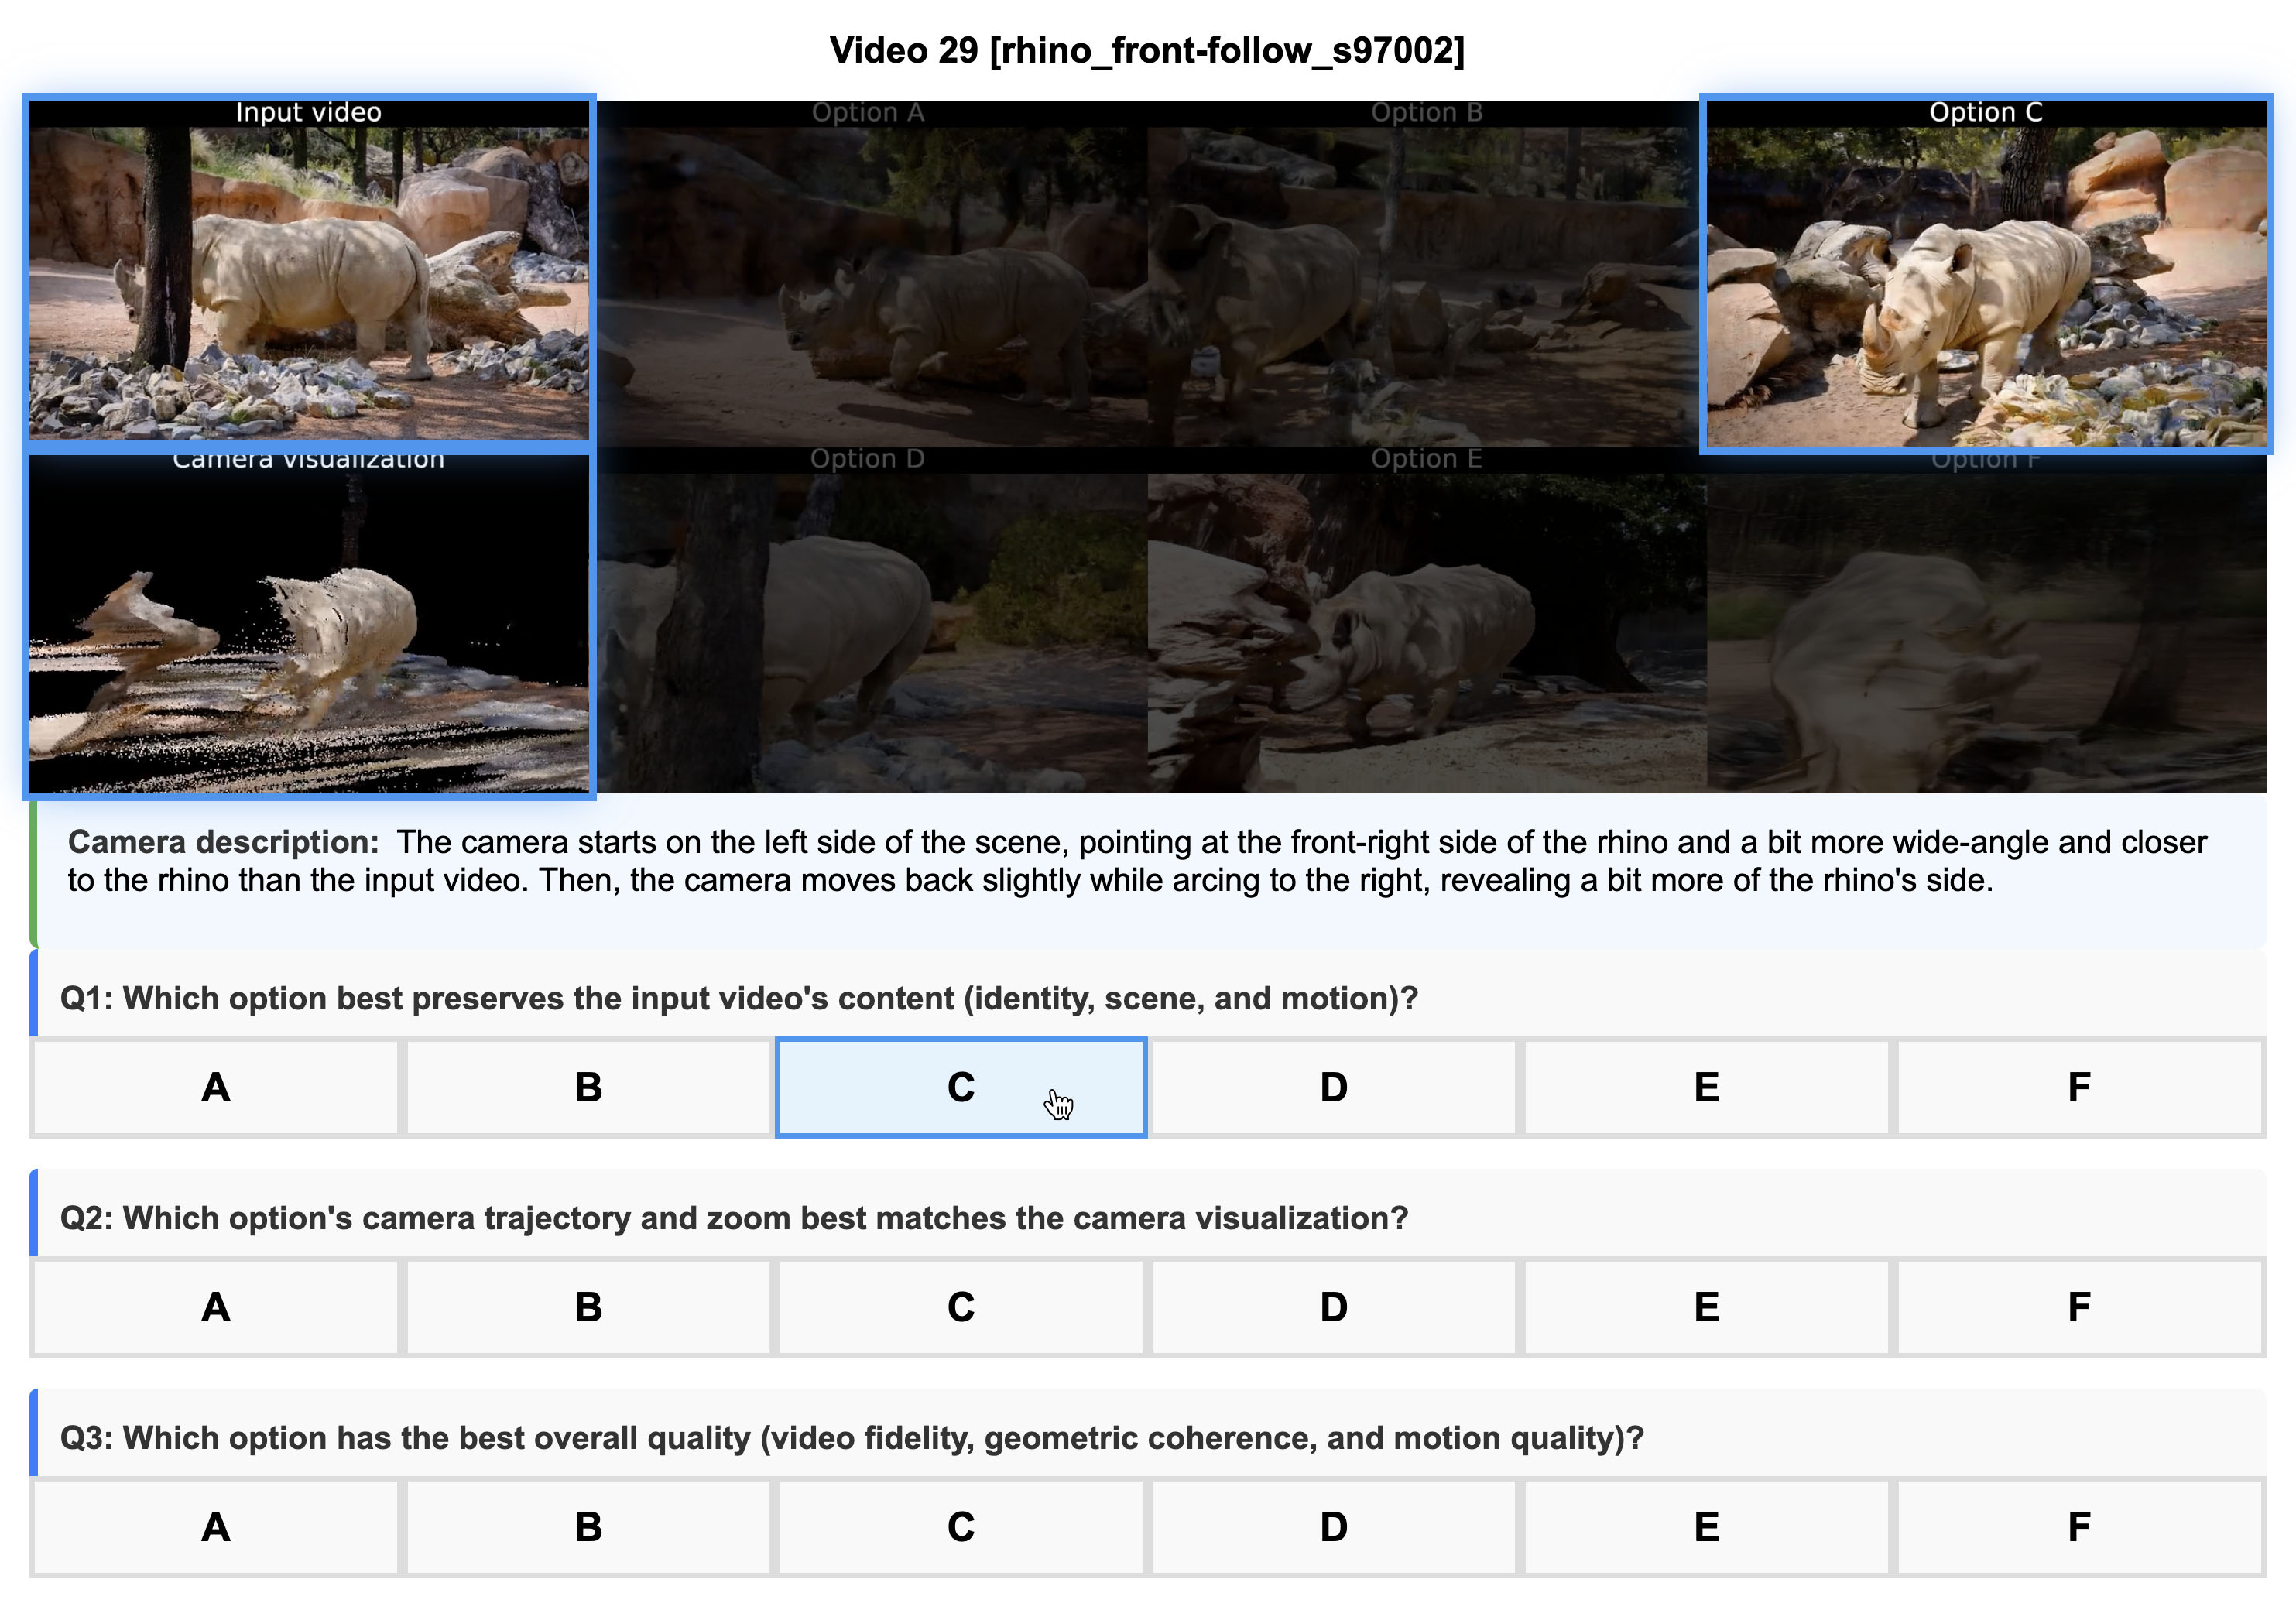
\includegraphics[width=0.49\textwidth]{figures/mid_res/user_study_rhino_hover.jpg}
    \caption{\Paragraphnoskip{User study} The left screenshot shows an example video-camera pair of our user study, where users are asked to select their preferred method/option on three dimensions: Source video preservation (Q1), camera control accuracy (Q2), and overall video fidelity (Q3). The right screenshot shows our user study UI highlighting the source video, point cloud render, and corresponding output video as users hover on each option. We also provide a camera description in addition to the point cloud render to communicate our intended target cameras. There are $30$ video-camera pairs in total in the user study, which was randomly selected from our $110$ video-camera pair evaluation dataset.}
    \label{fig:user_study}
\end{figure*}

\Paragraph{User study}
For our user study, we randomly select $30$ video-camera pairs from our evaluation dataset and invite $42$ participants to select their preferred method/option from \methodname and baseline video reshooting results. For each video-camera pair, we ask for the participants' preference on three dimensions: Source video content preservation (``Which option best preserves the input video's content (identity, scene, and motion)?''), camera control accuracy (``Which option's camera trajectory and zoom best matches the camera visualization?''), and overall video fidelity (``Which option has the best overall quality (video fidelity, geometric coherence, and motion quality)?''). For camera accuracy preference, we provide both the point cloud render and a short description of the intended target camera for each pair. The order of the methods is also randomized and anonymized for each pair. A screenshot of our user study can be found in Figure \ref{fig:user_study}.

\section{Quantitative evaluation metric details} \label{supp:quant_metrics}

\Paragraph{Camera control accuracy}
We perform camera control accuracy evaluation by comparing the predicted camera parameters $(\vec{R}_i^\gen, \vec{t}_i^\gen, \mathrm{FOV}_i^\gen)_{i=1}^T$ of the generated video and the target cameras $(\vec{R}_i^\tgt, \vec{t}_i^\tgt, \mathrm{FOV}_i^\tgt)_{i=1}^T$, where $\vec{R}, \vec{t}$ are the camera extrinsics and $\textrm{FOV}$ is the vertical field of view from the camera intrinsics. As the target camera parameters are represented in the source video's coordinate system, we first jointly reconstruct the camera poses of both the source and generated videos and then fit the source video part of the camera poses to the known source camera parameters using Umeyama alignment \cite{umeyama2002least}.

As many target videos generated by the baselines lack 3D consistency, traditional SFM and optimization-based methods like GLOMAP~\cite{pan2024glomap} used in prior works~\cite{CameraCtrl, bai2025recammaster} would fail to reconstruct the source and the target videos jointly. To obtain a fair camera accuracy evaluation, we adopt the learning-based 4D reconstruction method $\pi^3$~\cite{wang2025pi3} for joint reconstruction, which is also the same method used to reconstruct the source camera during inference. The evaluation metrics consist of the translation error, rotation error, and intrinsics error following~\cite{CameraCtrl, huang2025vipe} where
\begin{align}
    \text{RotErr}
    &= \frac{1}{T}\sum_{i=1}^{T}
    \arccos\!\left(
    \frac{\operatorname{tr}\!\left(\vec{R}_i^\tgt {\vec{R}_i^\gen}^{\!\top}\right) - 1}{2}
    \right) \, ,
    \\
    \text{TransErr}
    &= \frac{1}{T}\sum_{i=1}^{T}
    \left\| \vec{t}_i^\tgt - \vec{t}_i^\tgt \right\|_2^2 \, ,
    \\
    \text{IntrinsicsErr}
    &= \frac{1}{T}\sum_{i=1}^{T}
    \left\lvert \text{FOV}_i^{\text{tgt}} - \text{FOV}_i^\gen \right\rvert.
\end{align}

\Paragraph{3D consistency via reprojection error (RE@SG)} Traditional NVS metrics such as PSNR, SSIM, and LPIPS compare the generated images against a fixed-set of ground truth images. However, using them to evaluate a generative model unfairly penalizes plausible generations when they deviate from the ground truth in unseen regions, while being restrictive with evaluation datasets without ground truths. Pippo~\cite{kant2025pippo} proposed the Reprojection Error, which enables the evaluation of the 3D consistency of the generated scene from two given camera viewpoints (\ie known intrinsics and extrinsics) by utilizing LightGlue~\cite{lightglue} and SuperPoint~\cite{detone2018superpoint} for detecting 2D point matches, then triangulating them in 3D, and computing the re-projection between the 3D points and 2D correspondences. We utilize this metric to compare the 3D consistency of the baselines with that of \methodname.

\Paragraph{Novel-view synthesis}
We perform novel-view synthesis evaluation on the \texttt{iphone}~\cite{gao2022dycheck} dataset. Following TrajectorCrafter~\cite{yu2025trajcraft}, we evaluate on the five sequence subset without label errors. We use the moving camera as the source video, and the first static camera with continuous frames as the target. We also adopt the camera pose and depth map labels provided by Shape of Motion~\cite{wang2025shapeofmotion} for the point cloud input. For pixel-wise synthesis accuracy, we follow standard protocols~\cite{mildenhall2021nerf, kerbl20233d} and evaluate PSNR, SSIM, and LPIPS. As many pixels in the target video are invisible in the source video, we also compute masked metrics following Dycheck~\cite{gao2022dycheck} and evaluate mPSNR, mSSIM, and mLPIPS with covisibility masking to better compare the model's performance in preserving content in the source video. Finally, the standard novel view synthesis metrics only evaluate the frame-wise metrics without measuring the accuracy of the synthesized motion across frames. Thus, we further evaluate motion quality by comparing the ground-truth optical flow and the generated optical flow using end-point error (EPE). As ground-truth optical flow labels are not available in the \texttt{iphone} dataset, we use an off-the-shelf model, SEA-RAFT~\cite{wang2024sea}, to predict optical flow for both the ground-truth and generated videos.

\Paragraph{Video fidelity}
We evaluate the video fidelity, visual quality, and prompt alignment of \methodname\ and all baselines on our $110$ video-camera-pair dataset. For fidelity, we compute FID~\cite{heusel2017fid} and FVD~\cite{uterthiner2019fvd} between the generated videos and their corresponding source videos. We further use VBench~\cite{huang2024vbench} to assess multiple perceptual dimensions: aesthetic quality, predicted by an aesthetic model capturing frame-level layout, color richness, and visual harmony; imaging quality, which measures distortions such as over-exposure, blur, and noise; subject consistency, evaluating how stable the main subject remains across frames; background consistency, computed via CLIP feature similarity across frames to quantify temporal stability of the scene; and temporal style, which measures similarity between video features and a temporal-style description to assess motion-style coherence. In addition, we evaluate human anatomy using VBench-2.0~\cite{zheng2025vbench2}, which reports anomaly scores for the human body, hands, and face, reflecting a model’s ability to preserve anatomically consistent humans under novel camera trajectories. Finally, we use CLIP-T~\cite{radford2021clip} to measure prompt alignment.

\section{Ablation study} \label{supp:ablations}

We show samples for our ablations on no depth artifacts \& source video conditioning and no temporal persistence. Note that all ablations samples, including ones from our full method, are from checkpoints with fewer training steps than the final $672 \times 384$ checkpoint. We encourage viewing the ablation results on our \projectpage file, as it is difficult to show artifacts like temporal jittering and at times inaccurate camera control through still frames in the paper.

\begin{figure*}
    \centering
    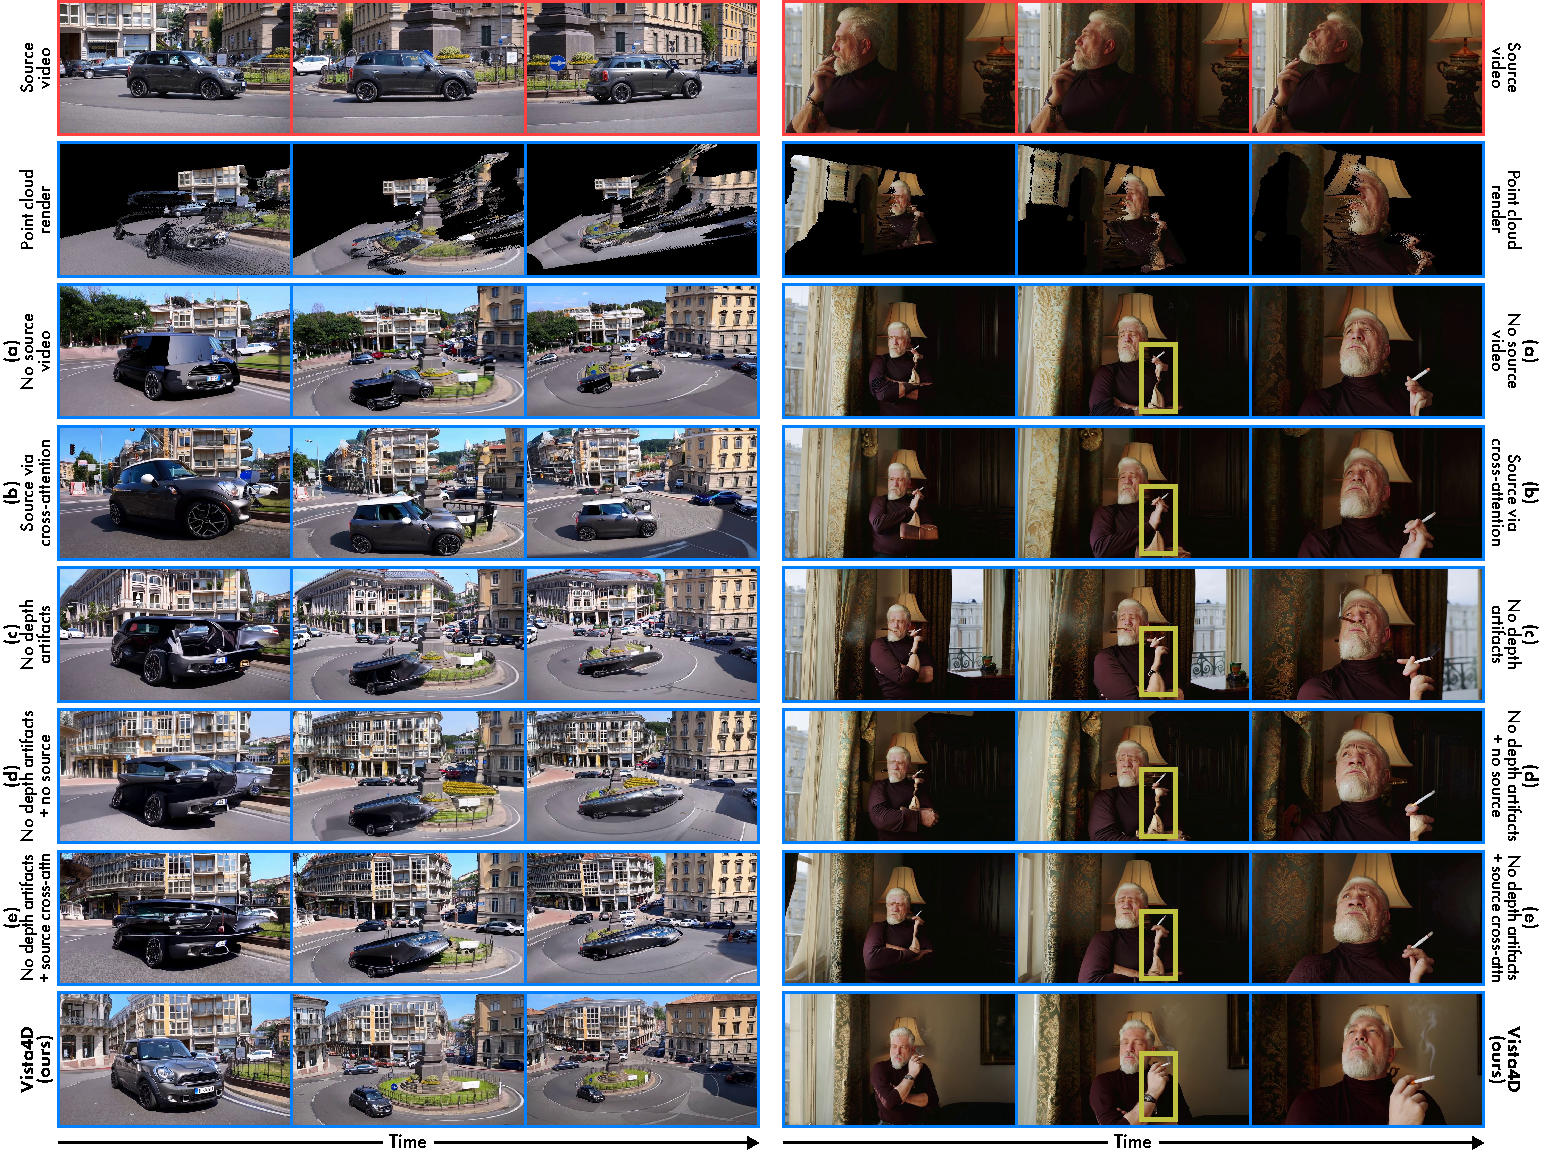
\includegraphics[width=\textwidth]{figures/mid_res/ablation_depth_source.pdf}
    \caption{\Paragraphnoskip{Ablation on depth artifacts and source video conditioning} We show ablation samples on training with depth artifacts (we simulate training without depth artifacts by always doing double reprojection for point cloud rendering \cite{yu2025trajcraft}) and source video conditioning (comparing our in-context/frame-concatenated source video conditioning with no source video and source video injected via cross-attention). Both examples above show 4D reconstruction artifacts carrying over to all ablations, such as on the car (left) or the man's arm and hand (right, highlighted by yellow boxes). Notably, though injecting the source video via cross-attention can at times correct point cloud artifacts, we find that cross-attention is often not adaptive enough, such as left (b) where the car is abnormally large despite the flying back camera. Both training without depth artifacts and in-context-conditioned source video also result in temporal jittering, but that is difficult to show as still frames in the paper. Thus, we encourage viewing these (and more) ablation samples as videos on our \projectpage.}
    \label{fig:ab_das}
\end{figure*}

\subsection{Depth artifacts and source video conditioning}

We show samples of our method with ablations in Figure \ref{fig:ab_das} on the following design choices:
\begin{enumerate}[label={\alph*)}]
    \item \textbf{No source video:} We take away source video conditioning and only condition on the point cloud render.
    \item \textbf{Source video via cross-attention:} Instead of in-context conditioning (\ie, self-attention through frame concatenation), we condition the source video via cross-attention following TrajectoryCrafter \cite{yu2025trajcraft}, as it is our only explicit-prior baseline which conditions on source videos in addition to point cloud renders.
    \item \textbf{No depth artifacts:} For the multiview dynamic dataset (MultiCamVideo dataset from ReCamMaster), instead of the point cloud render being rendered the source video in the cameras of the target video, we always do double reprojection to remove depth artifacts so the point cloud render is always spatially aligned with the target video.
    \item \textbf{No depth artifacts + no source video:} Combination of (b) and (a).
    \item \textbf{No depth artifacts + source cross-attn:} Combination of (c) and (a).
\end{enumerate}

We observe two major artifacts/problems when we remove depth artifacts and/or in-context/self-attention source video conditioning during training:
\begin{enumerate}
    \item \textbf{Geometry artifacts from imprecise depth estimation:} The model is unable to correct obvious depth estimation artifacts and thus produce output artifacts.
    \item \textbf{Temporal jittering:} One artifact of real-world depth estimation/4D reconstruction is temporal jittering of the resulting point cloud. Here, the model is unable to correct this jittering. Note that this is difficult to show as still frames in the paper, so we encourage viewing the ablation samples on our \projectpage.
\end{enumerate}
Figure \ref{fig:ab_das}, left exemplifies observation 1, where the 4D reconstruction artifacts on the car carried over to all ablations, except (b) where, though there are little depth artifacts, cross-attention was unable to properly transfer the car's geometry from the source video while ensuring its correct size with the camera flying back. Figure \ref{fig:ab_das}, right also shows observation 1, where every ablation (a) to (e) displays artifacts from depth estimation, especially around the man's right arm and hand. Observation 2 (temporal jittering) is difficult to present as still frames in the paper, so we encourage viewing the ablation samples, along with more ablation results, as videos on our \projectpage.

\begin{figure*}
    \centering
    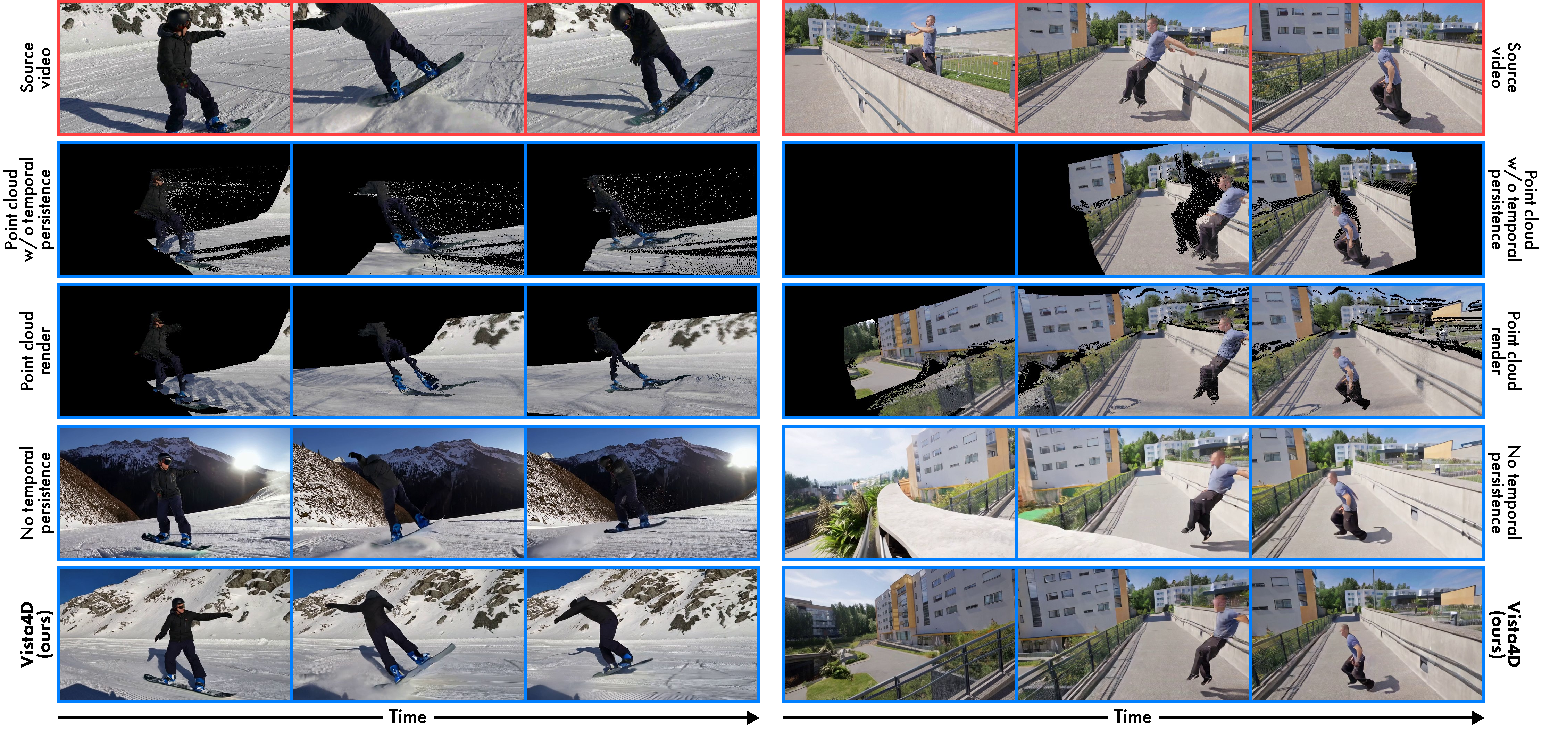
\includegraphics[width=\textwidth]{figures/mid_res/ablation_temporal.pdf}
    \caption{\Paragraphnoskip{Ablation on static pixel temporal persistence} We show ablation samples on training with and without static pixel temporal persistence. Both examples above show the no-temporal-persistence model struggling to preserve seen content from the source video, such as the snow and rock mountain (left) and the metal fence and the road beyond it (right). The model without temporal persistence also exhibits inaccurate camera control for both samples above, which is difficult to show as still frames in the paper. Thus, we encourage viewing these (and more) ablation samples as videos on our \projectpage.}
    \label{fig:ab_tp}
\end{figure*}

\subsection{Temporal persistence}

We show samples of our method trained with and without point cloud static pixel temporal persistence in Figure \ref{fig:ab_tp}, and we also show the corresponding point cloud conditioning with or without temporal persistence. We observe two major artifacts/problems when we remove temporal persistence:
\begin{enumerate}
    \item \textbf{Not preserving seen (static) content:} The model struggles to preserve seen content from the source video.
    \item \textbf{Imprecise camera control:} The model has less accurate camera control during target camera frames which have little overlap with the source video point cloud. Note that this can be difficult to show as still frames in the paper, so we encourage viewing the ablation samples on our \projectpage.
\end{enumerate}
Figure \ref{fig:ab_tp}, left encompasses observation 1, where the no-temporal-persistence model struggles to faithfully synthesize the snow and rock mountain behind the snowboarder as the per-frame point cloud render never explicitly sees it. Figure \ref{fig:ab_tp}, right also showcases observation 1, where the no-temporal-persistence model struggles to preserve the right side of the scene. Both examples also display observation 2, \ie, imprecise camera control, but that is difficult to show as still frames in the paper. Thus, we encourage viewing the ablation samples, along with more ablation results, as videos on our \projectpage.
